% !TeX document-id = {33927989-231d-43eb-85c8-eaa173529330}

% % % % % % % % % % % % % % % % % % % % % % % % % % % % % % % % % % % % % % % % %
%
% LaTex Documentation Template
%
% % % % % % % % % % % % % % % % % % % % % % % % % % % % % % % % % % % % % % % % %
% "THE BEER-WARE LICENSE" (Revision 42):
% Hannes Badertscher (hbaderts@hsr.ch) wrote this file. As long as you retain 
% this notice you can do whatever you want with this stuff. If we meet some day, 
% and you think this stuff is worth it, you can buy me a beer in return. 
% - Hannes Badertscher
% % % % % % % % % % % % % % % % % % % % % % % % % % % % % % % % % % % % % % % % %

% !TeX program = pdflatex
% !BIB program = biber
% !TeX encoding = utf8
% !TeX spellcheck = en


\RequirePackage[l2tabu, orthodox]{nag}   % Warnings for obsolete packages
\RequirePackage{etex}                    % Load extended TeX
\RequirePackage[utf8]{inputenc}          % Use UTF-8 as input encoding


% Document information
\newcommand*{\Lang}             	{en} % document language: de or en


\newcommand*{\Supervisor}          	{Prof. Stefan Keller}
\newcommand*{\Experte}          	{}
\newcommand*{\BetreuerA}        	{Nicola Jordan}
\newcommand*{\BetreuerB}          	{}
\newcommand*{\AuthorA}				{Conradin Kleinstein}
\newcommand*{\AuthorAMatrikel}	    {18-151-332}
\newcommand*{\AuthorB}				{Marco Fuchs}
\newcommand*{\AuthorBMatrikel}	    {18-156-703}
\newcommand*{\schoolDE}          	{OST - Ostschweizer Fachhochschule} 
\newcommand*{\schoolEN}          	{OST - Eastern Switzerland University of Applied Sciences} 
\newcommand*{\ModulInfo}     		{Seminar Database Systems}
\newcommand*{\Title}            	{Database Change Management Techniques\\by the Example of PostgreSQL}
\newcommand*{\Subtitle}            	{}
\newcommand*{\Studiengang}     		{Master of Science in Engineering}
\newcommand*{\Profile}     		    {Profile Data Science}
\newcommand*{\Semester}     		{Fall Semester \the\year{}}
\newcommand*{\Subject}      		{}
\newcommand*{\ThesisNr}         	{}
\newcommand*{\Keywords}         	{}
\newcommand*{\IsConfidential}   	{true}
\newcommand*{\Place}            	{St. Gallen}
\newcommand*{\TitleImage}       	{} % leave empty for no title image :frontmatter/Titelbild_bsp.jpg
\newcommand*{\Print}            	{true} % true for black links (print version), false for color links (pdf version)


% main header file
% % % % % % % % % % % % % % % % % % % % % % % % % % % % % % % % % % % % % % % % %
%
% LaTeX Documentation Template - Header File
%
% % % % % % % % % % % % % % % % % % % % % % % % % % % % % % % % % % % % % % % % %
% "THE BEER-WARE LICENSE" (Revision 42):
% Hannes Badertscher (hbaderts@hsr.ch) wrote this file. As long as you retain 
% this notice you can do whatever you want with this stuff. If we meet some day, 
% and you think this stuff is worth it, you can buy me a beer in return. 
% - Hannes Badertscher
% % % % % % % % % % % % % % % % % % % % % % % % % % % % % % % % % % % % % % % % %

% % % % % % % % % % % % % %
% Basic document setup\usepackage[T1]{fontenc}

\documentclass[
    11pt,                  % Font size
    final,
    parskip=half,          % Half a line skipped between paragraphs
    twoside,               % Two-sided document
    openright,             % Chapters start on right pages
    bibliography=totoc,    % Bibliography in ToC
    listof=totoc,          % LoF and LoT in ToC
]{scrreprt}[2015/09/15]    % Use current version of KOMA-Script


% Author and title of document
\author{\Author}
\title{\Title}
\date{\today}

% Load Fonts
%\usepackage[T1]{fontenc}                      % Use T1 encoding
%\usepackage[scaled=0.85]{berasans}            % Sans-serif: Bera Sans
%\usepackage[scaled=0.84]{beramono}            % Mono-space: Bera Mono
%\usepackage[sc]{mathpazo}                     % Serif: Palatino
%\linespread{1.05}                             % More linespread for Palatino

% Define text area
\typearea[10mm]{9}
\setlength{\marginparwidth}{25mm}
\textheight = 644pt
% Basic packages
\usepackage[final,activate={true,nocompatibility}]{microtype}    % Enable micro-typography
\usepackage{scrhack}             % Fixes koma-script incompatibilities
\usepackage{mparhack}            % Improved marginpar placement
\usepackage{float}				 % Precise Image Placement

% Load HSR colors

%marco -----------------


\newcommand\pro{\item[$+$]}
\newcommand\con{\item[$-$]}

\usepackage{lipsum} 

\usepackage[ruled,vlined]{algorithm2e}

\usepackage{enumitem}

\usepackage[table,xcdraw]{xcolor}
\usepackage{siunitx}
\usepackage{lscape} % querformat

\usepackage{trfsigns} % Transformation Symbol o---o \laplace and \Laplace

\usepackage[fleqn]{amsmath}

\newcommand{\vlaplace}[1][]{\mbox{\setlength{\unitlength}{0.1em}%
        \begin{picture}(10,20)%
            \put(3,2){\circle{4}}%
            \put(3,4){\line(0,1){12}}%
            \put(3,18){\circle*{4}}%
            \put(10,7){#1}
        \end{picture}%
    }%
}%

\newcommand{\vLaplace}[1][]{\mbox{\setlength{\unitlength}{0.1em}%
        \begin{picture}(10,20)%
            \put(3,2){\circle*{4}}%
            \put(3,4){\line(0,1){12}}%
            \put(3,18){\circle{4}}%
            \put(10,7){#1}
        \end{picture}%
    }%
}%                     



\usepackage{enumitem,amssymb}
\newlist{todolist}{itemize}{2}
\setlist[todolist]{label=$\square$}
\usepackage{pifont}
\newcommand{\cmark}{\ding{51}}%
\newcommand{\xmark}{\ding{55}}%
\newcommand{\done}{\rlap{$\square$}{\raisebox{2pt}{\large\hspace{1pt}\cmark}}%
    \hspace{-2.5pt}}
\newcommand{\wontfix}{\rlap{$\square$}{\large\hspace{1pt}\xmark}}

% % % % % % % % % % % % % %
\usepackage{xcolor}
\usepackage{header/HSRColors}
\usepackage{soul}


%Marco
\newcommand{\zerotext}[2][0pt]{\makebox[#1][l]{\qquad#2}}
\newcommand{\hlc}[2][yellow]{{%
            \colorlet{foo}{#1}%
            \sethlcolor{foo}\hl{#2}}%
}

\usepackage[a4paper]{geometry}

%---

% Header and footer
\usepackage[automark,headwidth=textwithmarginpar,footwidth=text,headsepline=0.4pt:textwithmarginpar]{scrlayer-scrpage}  % Custom header and footer
\pagestyle{scrheadings}
\renewcommand{\headfont}{\normalfont\sffamily}
\makeatletter
\renewcommand{\chaptermark}[1]{\markboth{\@chapapp~\thechapter~--~#1}{}}
\makeatother
\rohead{\rightmark}
\lehead{\leftmark}

% Bibliography
\usepackage[backend=biber,style=ieee]{biblatex}
\renewbibmacro*{bbx:savehash}{}                       % Don't abbreviate identical authors
\defbibheading{bibintoc}[\bibname]{%                  % Make bibliography title a chapter*
    \chapter*{#1}\markboth{#1}{#1}%
    \addcontentsline{toc}{chapter}{#1}%
}

% Glossary
\usepackage[toc]{glossaries}
\renewcommand{\glsnamefont}[1]{\makefirstuc{#1}}

% Index
\usepackage{imakeidx}
\makeindex[intoc,columnseprule]
\indexsetup{firstpagestyle=plain}    % Show header/footer on index page

% Aligned footnotes
\usepackage[hang]{footmisc}
\setlength{\footnotemargin}{1em}

% % % % % % % % % % % % % %
% Language stuff
\newcommand*{\LangDE}{de}
\ifx \Lang \LangDE
    \usepackage[english,ngerman]{babel}  % Main language: German
\else
    \usepackage[ngerman,english]{babel}  % Main language: English
\fi

% % % % % % % % % % % % % %
% Additional packages

% Date and time format
\usepackage{datetime}
\newdateformat{titledate}{\THEDAY.~\monthname\space\THEYEAR}

% Allow multicolumn document
\usepackage{multicol}

% Math
\usepackage{amsmath}
\usepackage{amssymb}
\usepackage{bm}

% Tables
\usepackage{multirow}
\usepackage{tabularx}
\usepackage{booktabs}

% Figures
\usepackage{pdfpages}
\usepackage{epstopdf}

% Listings - if you need advanced listings, switch to minted!
% Listing styles by by github.com/rnestler / github.com/dkoeppel for github.com/HSR-Stud/header
% Licensed under CC-BY-NC-SA

\ifx\GUARDlistings\undefined		% include guard
\def\GUARDlistings{}

\usepackage{listings}

	\lstdefinestyle{Java}{ numbers=left,
	  belowcaptionskip=1\baselineskip,
	  breaklines=true,
	  frame=L,
	  xleftmargin=\parindent,
	  language=Java,
	  showstringspaces=false,
	  basicstyle=\footnotesize\ttfamily,
	  keywordstyle=\bfseries\color{green!40!black},
	  commentstyle=\itshape\color{purple!40!black},
	  identifierstyle=\color{blue},
	  stringstyle=\color{orange},
	  numberstyle=\ttfamily\tiny
	}
	
	\lstdefinestyle{SQL}{
	  numbers=none,
	  belowcaptionskip=1\baselineskip,
	  breaklines=true,
	  xleftmargin=\parindent,
	  language=SQL,
	  showstringspaces=false,
	  basicstyle=\footnotesize\ttfamily,
	  keywordstyle=\bfseries\color{green!40!black},
	  commentstyle=\itshape\color{purple!40!black},
	  identifierstyle=\color{blue},
	  stringstyle=\color{orange},
	}
	
	\lstdefinestyle{C}{
	  numbers=left,
	  belowcaptionskip=1\baselineskip,
	  breaklines=true,
	  frame=L,
	  xleftmargin=\parindent,
	  language=C,
	  showstringspaces=false,
	  basicstyle=\footnotesize\ttfamily,
	  keywordstyle=\bfseries\color{green!40!black},
	  commentstyle=\itshape\color{purple!40!black},
	  identifierstyle=\color{blue},
	  stringstyle=\color{orange},
	  numberstyle=\ttfamily\tiny
	}
	
	\lstdefinestyle{Cpp}{
	  numbers=left,
	  belowcaptionskip=1\baselineskip,
	  breaklines=true,
	  frame=L,
	  xleftmargin=\parindent,
	  language=C++,
	  showstringspaces=false,
	  basicstyle=\footnotesize\ttfamily,
	  keywordstyle=\bfseries\color{green!40!black},
	  commentstyle=\itshape\color{purple!40!black},
	  identifierstyle=\color{blue},
	  stringstyle=\color{orange},
	  numberstyle=\ttfamily\tiny
	}
	
	\lstdefinestyle{Csharp}{
	  numbers=left,
	  belowcaptionskip=1\baselineskip,
	  breaklines=true,
	  frame=L,
	  xleftmargin=\parindent,
	  language=[Sharp]C,
	  showstringspaces=false,
	  basicstyle=\footnotesize\ttfamily,
	  keywordstyle=\bfseries\color{green!40!black},
	  commentstyle=\itshape\color{purple!40!black},
	  identifierstyle=\color{blue},
	  stringstyle=\color{orange},
	  numberstyle=\ttfamily\tiny
	}
	
	
	\lstdefinestyle{Matlab}{
	  numbers=left,
	  belowcaptionskip=1\baselineskip,
	  breaklines=true,
	  frame=L,
	  xleftmargin=\parindent,
	  language=Matlab,
	  showstringspaces=false,
	  basicstyle=\footnotesize\ttfamily,
	  keywordstyle=\bfseries\color{green!40!black},
	  commentstyle=\itshape\color{purple!40!black},
	  identifierstyle=\color{blue},
	  stringstyle=\color{orange},
	  numberstyle=\ttfamily\tiny
	}
	
	\definecolor{mygreen}{rgb}{0,0.6,0}
	\definecolor{mygray}{rgb}{0.5,0.5,0.5}
	\definecolor{mymauve}{rgb}{0.58,0,0.82}
	\definecolor{grund}{gray}{0.9} 

	
\lstset{ 
  backgroundcolor=\color{grund},   % choose the background color; you must add \usepackage{color} or \usepackage{xcolor}; should come as last argument
  basicstyle=\footnotesize,        % the size of the fonts that are used for the code
  breakatwhitespace=true,         % sets if automatic breaks should only happen at whitespace
  breaklines=true,                 % sets automatic line breaking
  captionpos=b,                    % sets the caption-position to bottom
  commentstyle=\color{mygreen},    % comment style
  deletekeywords={...},            % if you want to delete keywords from the given language
  escapeinside={\%*}{*)},          % if you want to add LaTeX within your code
  extendedchars=true,              % lets you use non-ASCII characters; for 8-bits encodings only, does not work with UTF-8
  firstnumber=1,                		% start line enumeration with line 1000
  frame=single,	                   % adds a frame around the code
  keepspaces=false,                 % keeps spaces in text, useful for keeping indentation of code (possibly needs columns=flexible)
  keywordstyle=\color{blue},       % keyword style
  language=Python,                 		% the language of the code
  morekeywords={*,...},            % if you want to add more keywords to the set
  numbers=left,                    % where to put the line-numbers; possible values are (none, left, right)
  numbersep=8pt,                   % how far the line-numbers are from the code
  numberstyle=\tiny\color{mygray}, % the style that is used for the line-numbers
  rulecolor=\color{black},         % if not set, the frame-color may be changed on line-breaks within not-black text (e.g. comments (green here))
  showspaces=false,                % show spaces everywhere adding particular underscores; it overrides 'showstringspaces'
  showstringspaces=false,          % underline spaces within strings only
  showtabs=false,                  % show tabs within strings adding particular underscores
  stepnumber=2,                    % the step between two line-numbers. If it's 1, each line will be numbered
  stringstyle=\color{mymauve},     % string literal style
  tabsize=2	                   % sets default tabsize to 2 spaces
  %title=\lstname                   % show the filename of files included with \lstinputlisting; also try caption instead of title
}
	
	


\fi
% \usepackage[newfloat, chapter]{minted}
% \usemintedstyle{friendly}

% Si Units
\usepackage{siunitx}
\sisetup{detect-all,sticky-per,per-mode=symbol}

% Quotation marks
\usepackage{csquotes}
\setquotestyle[quotes]{german}

%Picutures
%\usepackage{graphicx}

% % % % % % % % % % % % % %
% Numbering and captions
\numberwithin{equation}{chapter}
\numberwithin{figure}{chapter}
\numberwithin{table}{chapter}

% Setup captions
\usepackage{caption}[2008/08/24]
\usepackage{subcaption}
\setkomafont{captionlabel}{\scshape\color{HSRBlue}}
\captionsetup{labelsep=quad}

% Setup toc and section numbering depth
\setcounter{tocdepth}{2}
\setcounter{secnumdepth}{4}

%marco
%\usepackage[table,xcdraw]{xcolor}
% % % % % % % % % % % % % %
% Hyperref setup
\usepackage[
    pdftitle={\Title},
    pdfauthor={\AuthorA \AuthorB},
    pdfkeywords={\Keywords},
    pdflang={\Lang},
    pdfpagemode=UseOutlines,  % Show outlines when opening pdf.
    pdfdisplaydoctitle=true,  % Show document title in pdf viewer.
    pdfcreator={LaTeX with hyperref and KOMA-Script},
    colorlinks=true,
    linkcolor=HSRBlue,
    citecolor=HSRBlue,
    filecolor=HSRBlue,
    urlcolor=HSRBlue,
    bookmarksnumbered=true
]{hyperref}



% If \Print=true, then make all links black for nicer print
\providecommand*{\True}{true}
\ifx \Print \True
    \hypersetup{hidelinks}
\fi

% Nameref setup
\usepackage{zref-titleref}
\makeatletter
\newcommand*{\currentname}{\zref@getcurrent{title}}
\makeatother


% Set reference names
\addto\extrasenglish{% English
    \renewcommand*{\figureautorefname}{Fig.}             % fig:
    \renewcommand*{\tableautorefname}{Tab.}              % tab:
    \renewcommand*{\equationautorefname}{Eq.}            % eq:
    \renewcommand*{\chapterautorefname}{Chp.}            % chp:
    \renewcommand*{\sectionautorefname}{Sec.}            % sec:
    \renewcommand*{\subsectionautorefname}{Sec.}         % subsec:
    \providecommand*{\listingautorefname}{Listing}
}
\addto\extrasngerman{% German
    \renewcommand*{\figureautorefname}{Abb.}             % fig:
    \renewcommand*{\tableautorefname}{Tab.}              % tab:
    \renewcommand*{\equationautorefname}{Gl.}            % eq:
    \renewcommand*{\chapterautorefname}{Kapitel}            % chp:
    \renewcommand*{\sectionautorefname}{Kapitel}            % sec:
    \renewcommand*{\subsectionautorefname}{Kapitel}         % subsec:
    \renewcommand*{\subsubsectionautorefname}{Kapitel}      % subsubsec:
}

% % % % % % % % % % % % % %
% Marginpar setup
\usepackage{ragged2e}
\newcommand*{\oldmarginpar}{}
\let\oldmarginpar\marginpar
\renewcommand*{\marginpar}[1]{%
    \leavevmode\oldmarginpar%
    [\RaggedLeft\scshape\footnotesize\textcolor{HSRBlue}{\hspace{0pt}#1}]%
    {\RaggedRight\scshape\footnotesize\textcolor{HSRBlue}{\hspace{0pt}#1}}%
}

% % % % % % % % % % % % % %
% Itemize items
\newcommand{\hsrlistitemi}{\textcolor{HSRBlue}{\raisebox{.3ex}{\tiny$\blacksquare$}}}
\newcommand{\hsrlistitemii}{\textcolor{HSRLightGray}{\raisebox{.3ex}{\tiny$\blacksquare$}}}
\newcommand{\hsrlistitemiii}{\textcolor{HSRLightGray}{\raisebox{.3ex}{\tiny$\blacktriangleright$}}}

\renewcommand{\labelitemi}{\hsrlistitemi}
\renewcommand{\labelitemii}{\hsrlistitemii}
\renewcommand{\labelitemiii}{\hsrlistitemiii}

% % % % % % % % % % % % % %
% Chapter headings
\makeatletter
% In Document titles
\renewcommand{\@makechapterhead}[1]{%
    \vspace*{10\p@}%
    \hfill%
    \begin{minipage}[b]{9cm}%
        \raggedleft%
        \sffamily\huge\textbf{\thechapter}
        \sffamily\huge\textbf{#1}%

    \end{minipage}%
    \quad%
    %    {\fontsize{60pt}{3em}\selectfont\sffamily\textbf{\textcolor{HSRBlue}{\thechapter}}}%
    \vskip 5\p@%
    \noindent\makebox[\textwidth-2em][l]{\textcolor{HSRBlue}{\rule{\paperwidth-\oddsidemargin-\hoffset-1in}{0.7pt}}}%
    \vskip 25\p@%
    \normalfont\normalsize%
}

\renewcommand{\@makeschapterhead}[1]{%
    \vspace*{10\p@}%
    \hfill%
    \begin{minipage}[b]{9cm}%
        \raggedleft%
        \sffamily\huge\textbf{#1}%
    \end{minipage}%
    \vskip 5\p@%
    \noindent\makebox[\textwidth-2em][l]{\textcolor{HSRBlue}{\rule{\paperwidth-\oddsidemargin-\hoffset-1in}{0.7pt}}}%
    \vskip 25\p@%
    \normalfont\normalsize%
}
\makeatother

% % % % % % % % % % % % % %
% Appendix page + toc entry
\usepackage{appendix}

\makeatletter
%\renewcommand{\@chap@pppage}{%
%    \clear@ppage
%    \thispagestyle{empty} % this was 'plain' before
%    \if@twocolumn\onecolumn\@tempswatrue\else\@tempswafalse\fi
%    \null\vfil
%    \markboth{}{}%
%    {%
%        \centering
%        \interlinepenalty \@M
%        \normalfont
%        %\Huge \bfseries\sffamily \appendixpagename\par % this was rmfamily 
%        \Huge \bfseries\sffamily Anhang \par % this was rmfamily
%    }%
%    \if@dotoc@pp
%        \addappheadtotoc
%    \fi
%    \vfil\newpage
%    \if@twoside
%        \if@openright
%            \null
%            \thispagestyle{empty}%
%            \newpage
%        \fi
%    \fi
%    \if@tempswa
%        \twocolumn
%    \fi
%}
\makeatother

% % % % % % % % % % % % % %
% TikZ and PGF Plots
\usepackage{tikz}
\usepackage{pgfplots}

% Tikz Libraries
\usetikzlibrary{positioning}

% Use Sans-Serif family in TikZ graphics
\tikzset{font=\sffamily}

% If there are many TikZ images, make them external.
% Note: you'll have to call pdflatex with the -shell-escape flag!
%\usetikzlibrary{external}
%\tikzexternalize[prefix=tikz/]

% Create cycle list with HSR colors
\pgfplotscreateplotcyclelist{hsrcolorlist}{%
    HSRSchwarz,every mark/.append style={solid,fill=HSRSchwarz}     \\%
    HSRBlue,every mark/.append style={solid,fill=HSRBlue}           \\%
    HSRHematite,every mark/.append style={solid,fill=HSRHematite}   \\%
    HSRBasswood,every mark/.append style={solid,fill=HSRBasswood}   \\%
}
% Set default cycle list for plots
\pgfplotsset{cycle multi list={mark list\nextlist hsrcolorlist}}

% Set default cycle list for bar plots
\pgfplotsset{
    /pgfplots/bar cycle list/.style={/pgfplots/cycle list={%
                    {HSRBlue,fill=HSRBlue60,mark=none},%
                    {HSRHematite,fill=HSRHematite60,mark=none},%
                    {HSRBasswood,fill=HSRBasswood60,mark=none},%
                }}
}

% % % % % % % % % % % % % %
% ToDo notes
\newcommand{\todonotecolor}{red}

% Small TODO note
\newcommand{\todonote}[1]{%
    \marginpar{\textcolor{\todonotecolor}{ToDo}}%
    \colorbox{red}{\sffamily\textcolor{white}{#1}}%
    \PackageWarning{ToDo:}{#1!}%
}

% Large TODO note
\newcommand{\todo}[1]{%
    \marginpar{\textcolor{\todonotecolor}{ToDo}}%
    \colorbox{red}{\parbox{\linewidth}{\sffamily\textcolor{white}{#1}}}%
    \PackageWarning{ToDo:}{#1!}%
}

% Command: Citation needed!
\newcommand{\citationneeded}{%
    \marginpar{\textcolor{\todonotecolor}{ToDo}}%
    \sffamily\textcolor{red}{$^\text{[Citation needed]}$}
    \PackageWarning{ToDo:}{Citation needed!}%
}

\usepackage{calc}
\usepackage{color}
\definecolor{mygreen}{rgb}{0,0.6,0}
\definecolor{mygray}{rgb}{0.5,0.5,0.5}
\definecolor{mymauve}{rgb}{0.58,0,0.82}
\definecolor{grund}{gray}{0.9}

\newcommand{\env}[1]{\texttt{#1}}
\newcommand{\command}[1]{\texttt{#1}}
\newcommand{\package}[1]{\texttt{\itshape#1}}

\usepackage{gensymb}
\usepackage{cleveref}

% % % % % % % % % % % % % % % % % % % % % % % % % % % % % % % % % % % % % % % % %
%
% Glossary entries
%
% % % % % % % % % % % % % % % % % % % % % % % % % % % % % % % % % % % % % % % % %

\makenoidxglossaries

% Glossary entries
\newglossaryentry{SQLg}{name={sturctured query language}, description={Domain specific language used in programming designed for managing data held in a relational database management system. \cite{SQLWiki}}}

\newglossaryentry{JAVAg}{name={Java}, description={General purpose programming language \cite{JavaWiki}}}

\newglossaryentry{JDBC}{name=java database connectivity, description={JDBC is a Java API that allows Java programs to connect to and interact with a database}}

\newglossaryentry{BLOB}{name=binary large object, description={Data type that can store large amounts of binary data such as images or videos in databases or other types of storage sytems \cite{Blob2022}}}

\newglossaryentry{CLOB}{name=character large object, description={Data type that can store large amounts of character data such as a long text \cite{Blob2022}}}


% Acronyms
\newglossaryentry{SQL}{type=\acronymtype, 
	name={SQL}, 
	description={Structured Query Language}, 
	first={structured query language (SQL) \glsadd{SQLg}}, see=[Glossary:]{SQLg}}

\newacronym{GUI}{GUI}{graphical user interface}
\newacronym{DB}{DB}{database}
\newacronym{DDL}{DDL}{data definition language}
\newacronym{DML}{DML}{data manipulation language}
\newacronym{CLI}{CLI}{command line interface}
\newacronym{VCS}{VCS}{version control system}


\newacronym{svm}{SVM}{support vector machine}
\newacronym{API}{API}{application programming interface}
\newacronym{GNN}{GNN}{Graph Neural Network}
\newacronym{CI}{CI}{Continuous Integration}
\newacronym{DBA}{DBA}{database administrator}
%\makeglossaries

\bibliography{frontmatter/bibliograpy.bib}

\setlength{\textheight}{644pt}


% % % % % % % % % % % % % %
\begin{document}

% Frontmatter
\pagenumbering{roman}

\begin{titlepage}
	 \newgeometry{top=2cm, left=2.5cm, right=2.5cm, bottom=2.5cm}

	%	\ifnum\value{documentfakultaet}=0
	%	\definecolor{strich}{cmyk}{0,.97,.92,.11} % Bau-Wasser-Boden
	%	\fi\ifnum\value{documentfakultaet}=1
	%	\definecolor{strich}{rgb}{0,.62,.89} % Informatik
	%	\fi


	% \begin{flushleft}
	% 	\includegraphics[scale=0.9]{header/ost_logo1}\\
	% \end{flushleft}

	% \newgeometry{top=2cm, right=2.5cm}
	% \begin{flushright}
	% 	
\includegraphics[scale=0.6]{header/mse-full-grey-large}\\
	% \end{flushright}

 	\noindent
	\vspace{-2cm} 
	\begin{center}
		\begin{minipage}{0.5\textwidth}%
			\begin{flushleft}
				
\includegraphics[width=1.0\textwidth]{header/mse-full-grey-large}%
			\end{flushleft}
		\end{minipage}\hfill
		\begin{minipage}{0.5\textwidth}%
			\begin{flushright}
				
\includegraphics[scale=0.8]{header/ost_logo_enlish}\\
			\end{flushright}
		\end{minipage}
	\end{center}

	
	% 
\includegraphics[scale=0.6]{header/mse-full-grey-large}\hfill\includegraphics[scale=0.9]{header/ost_logo1}

	%	\begin{flushleft}
	\center
	\vspace{2cm}
	{\color{OSTpurple}\fontsize{21}{20}{\textbf{\Title}}}\\
	\vspace{0.5cm}
	\color{black}
	{\fontsize{15}{20}{\textsf{\Subtitle}}}\\
	\vspace{3cm}
	

	
	\color{black}
	
	{\ModulInfo}\\
	{\Studiengang}\\
	{\Profile}\\
	{\Semester}\\

	\vspace{1.5cm}
	
	Authors\\
	
	{\textbf\AuthorA}\\
	{\small Matriculation No. \AuthorAMatrikel}\\
	
	\vspace{.5cm}
	{\textbf\AuthorB}\\
	{\small Matriculation No. \AuthorBMatrikel}\\




	\vspace{1.5cm}

	\color{black}



	\color{black}
	Supervisor:\\ \textbf{\Supervisor}\\
		
		


	\vspace{3.5cm}

  
	\titledate\today

	 
	 \vfill
	 \begin{flushright}
	 	\vfill
	 	\color{OSTpurple}\small\textsf{
	 		Buchs $ \cdot $ St. Gallen $ \cdot $ \textbf{Rapperswil}
	 	}
	 \end{flushright}
	

	% \newgeometry{top=2cm, right=2.5cm}
	% \begin{flushright}
	% 	
\includegraphics[scale=0.6]{header/mse-full-grey-large}\\
	% \end{flushright}

	% \begin{minipage}{0.5\textwidth}%
	% 	\begin{flushleft}
	% 		\titledate\today
	% 	\end{flushleft}
	% \end{minipage}\hfill
	% \begin{minipage}{0.5\textwidth}%
	% 	\begin{flushright}
	% 		\vfill
	% 		\color{OSTpurple}\small\textsf{
	% 			Buchs $ \cdot $ St. Gallen $ \cdot $ \textbf{Rapperswil}
	% 		}
	% 	\end{flushright}
	% \end{minipage}
	
	

\end{titlepage}

\restoregeometry


%\cleardoublepage
\markleft{\abstractname}
\pdfbookmark[1]{Abstract}{abstract}

\chapter*{Abstract}
\marginpar{Ausgangslage}%
The abstract gives a concise overview of the work you have done. The reader shall be able to decide whether the work which has been done is interesting for him by reading the abstract. Provide a brief account on the following questions:

\begin{itemize}
	\item What is the problem you worked on? (Introduction)
	\item How did you tackle the problem? (Materials and Methods)
	\item What were your results and findings? (Results)
	\item Why are your findings significant? (Conclusion)
\end{itemize}

The abstract should approximately cover half of a page, and does generally not contain citations.
 
\marginpar{Vorgehen}%
\url{https://www.jacquelinedrost.com/thesis-structure/}\\
Structure thesis: Introduction, Related Work, Background, Approach, Implementation, Evaluation/Results, Discussion, Future Work\\


\marginpar{Ergebnisse}%
\lipsum[1]


\tableofcontents


% Main part
\cleardoublepage
\pagenumbering{arabic}


% !TeX spellcheck = en_US

\chapter{Introduction}

The following sections provide a brief introduction to database change
management. This includes short summary of its history and focuses on
the benefits database change management provides.

\section{Problem Statement and Benefits}%


\section{State of the Art}%
This section aims to answer the question of what is state of the art in database change management techniques.

\section{Available tools}%
This section will provide an overview of available change management tools.
The list of tools should include the available programming languages, price / availability
and the main advantage over their competitors.

\section{Overview}%
This section will provide an overview of thesis.


\newpage

% !TeX spellcheck = en_US

\chapter{Introduction to Flyway}


\section{Overview}
\marginpar{Information}%
Flyway is a tool that makes database migrations easy and provides version control for databases. It is a multi-platform and cross-database tool with support for over 20 databases.
Axel Fontaine from Google Code created Flyway in 2010 and was acquired by Redgate Software in 2019. Flyway is currently at the 9th version when creating this work. The creator was looking for a simple method to implement database changes quickly and directly in \gls{SQLg}. His main goal was to include database changes as part of the software deployment process \cite{Robles2021}.
Flyway uses the freemium business model. The basic version is free and open source \cite{Fontaine2010} and additionally, there is a paid Teams or Enterprise Edition available.

With Flyway, migration files are written in either with \gls{SQLg} (database-specific syntax (such as PL/SQL, T-SQL) or \gls{JAVAg} (for advanced data transformations or dealing with LOBs). Flyway can connect to databases hosted in on-premises or cloud environments, thanks to the included JDBC driver library that is shipped with the tool. It runs on all modern platforms, such as Linux, Mac or Windows.  \cite{Dillon2022} \cite{DBMSTools}


\marginpar{Migrations \cite{Parsick2018} \cite{Lukonin2017}}%
There are four possibilities of migrations as shown in \autoref{tab:migration_types}. There are versioned migrations with scripts with a unique meanings, executed only once. These versioned migrations are mainly used for Data Definition Language (DDL), like creating or modifying a table.

Repeatable migration scripts do not have a version number. These are always if their checksum changes and after the versioned migrations are applied. Typical applications for repeatable tasks are importing base data, rebuilding views or indexes, and adding permissions or other maintenance tasks.

\begin{table}[h]
	\centering
	\begin{tabularx}{8cm}{X c c}
		Basis & Versioned & Repeatable \\ \toprule
		SQL based & \checkmark & \checkmark \\
		Java based & \checkmark & \checkmark \\
	\end{tabularx}
	\caption{Migration Types - Based on Parsick et al. \cite{Parsick2018}}
	\label{tab:migration_types}
\end{table}

\marginpar{SQL Migrations}%
Flyway developers can migrate changes directly with \gls{SQLg}. Per default, Flyway takes the database migrations from the directory \textit{sql}.
These \gls{SQLg} migration files have to follow the naming convention:

\begin{center}
\begin{tabularx}{8cm}{r l}
Versioned & \texttt{\textcolor{blue}{V}\textcolor{green}{1\_1\_1}\textcolor{red}{\_\_}\textcolor{orange}{create\_table}.sql}\\
Repeatable & \texttt{\textcolor{blue}{R}\textcolor{red}{\_\_}\textcolor{orange}{create\_table}.sql}\\
\end{tabularx}
\end{center}

\begin{flushright}
\textcolor{blue}{Prefix}\\
\textcolor{green}{Version}\\
\textcolor{red}{Seperator (two underscores)}\\
\textcolor{orange}{Description}\\
\end{flushright}

\todo{Table and Legend are ugly.}

These \gls{SQL} scripts can have several rows and allow all database-specific syntax, including comments. These \gls{SQL} migrations are mainly used for DDL changes such as create, alter, and drop for simple data changes.

\marginpar{Java Migrations}%
Unlike changes in \gls{SQL}, \gls{JAVAg} changes are more for BLOB or CLOB changes or for progressive changes to an extensive data set like recalculations. The naming convention is similar; only the ending differs.

\todo{Add BLOB, CLOB to glossary.}

\begin{center}
	\begin{tabularx}{8cm}{r l}
		Versioned & \texttt{\textcolor{blue}{V}\textcolor{green}{1\_1\_1}\textcolor{red}{\_\_}\textcolor{orange}{create\_table}.java}\\
		Repeatable & \texttt{\textcolor{blue}{R}\textcolor{red}{\_\_}\textcolor{orange}{create\_table}.java}\\
	\end{tabularx}
\end{center}

\marginpar{Advanced Changes\\ \cite{Parsick2018}}%
Some migration steps need user intervention, for example, creating a materialized view. This functionality is provided by flyway with callback functions. 

\begin{figure}[H]
	\centering
	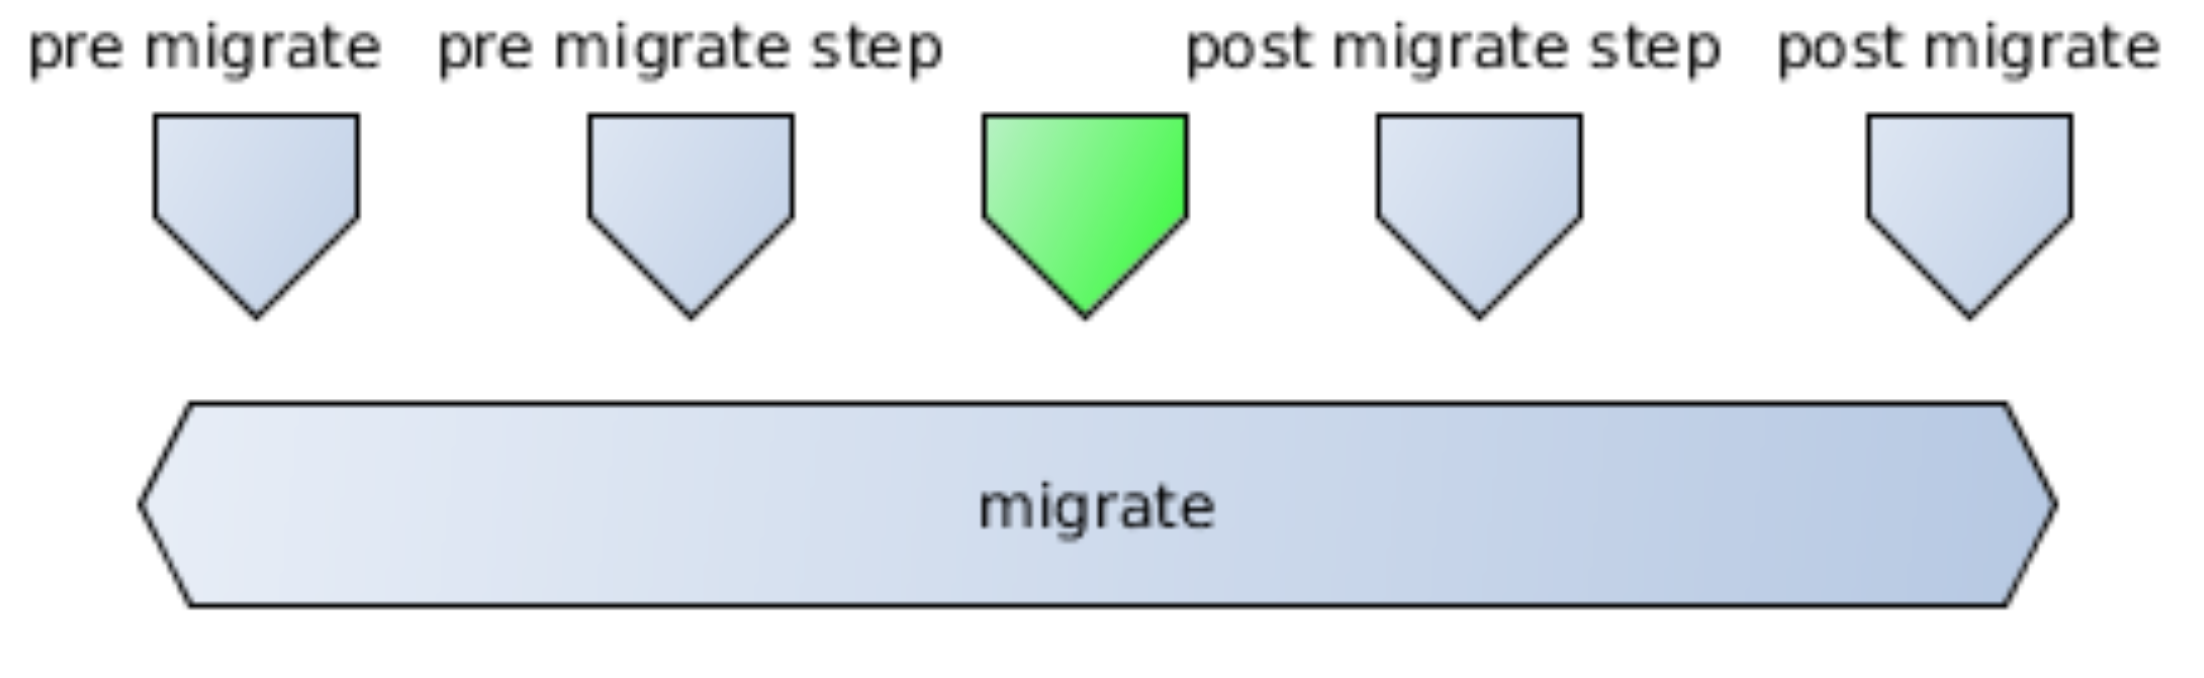
\includegraphics[width=0.6\textwidth]{./chapters/intro_flyway/images/advanced_migrations}
	\caption[Flyway Lifecycle - Source: \cite{Parsick2018}]{Flyway Lifecycle}
	\label{fig:advanced_migrations}
\end{figure}

There are several options for the execution times. The defined naming convention recognizes these times. The callbacks can be written in \gls{SQLg} or \gls{JAVAg}. 

\begin{lstlisting}[caption=SQL Callback Functions for Flyway - Source: \cite{FlywayCallbacks}]
BeforeMigrate.sql
BeforeEachMigrate.sql
AfterEachMigrate.sql
AfterMigrate.sql
\end{lstlisting}

If the task needs to be more powerful or flexible, \gls{JAVAg} callbacks can be formulated as follows:
\begin{lstlisting}[caption=Java Callback Functions before clean - Source: \cite{FlywayCallbacks}]
public interface FlywayCallback {
	/**
	* Runs before the tasks executes
	* by avoiding unnecessary connection state setups for events 
	* that will not be handled anyway.
	* @param valid connection to a database
	*/
	void beforeClean(Connection connection);
}
\end{lstlisting}
Other callback function can be formulated with the same name as the SQL-functions.

\marginpar{Dealing with Hotfixes\\ \cite{Lukonin2017}}%
To apply Flyway migrations out of order and fill in any gaps, activate the \textit{outOfOrder} property. This functionality is useful when the production environment is older, but the development and test environments are already at a new version. Hotfixes in between can then be applied by activating the \textit{outOfOrder} property. In addition, as described in the introduction \autoref{best_practices}, if you have multiple developers working on different branches, it may be helpful to enable the \textit{outOfOrder} property to allow for more flexibility in the migration and branching process.


\marginpar{Flyway Teams \cite{FlywayTeams}}%
The Pro-Version of Flyway is called Flyway Teams. This pro version costs (as of creation of this work) 447€ per user per year. It offers:
\begin{itemize}
	\item Additional migration controls
	\item Protect against failed deployments
	\item Professional technical support from Redgate
	\item Support for older DB versions
	\item Built-in Git client and object-level versioning
\end{itemize}

Compared to the team version, the free, open-source version includes the core functionalities with desktop \gls{GUI} support for only the current database versions and support through the community. The core functionalities include the six basic commands: migrate, clean, info, validate, baseline and repair.

A comparison between the Flyway editions can be found here \autoref{label}.\\
\todo{Liste einfügen in Anhang}

\marginpar{Community}%
Stars on GitHub: 6'900 (27. December 2022)\\
Tags on StackOverflow: 2,118 (31. December 2022)\\

\marginpar{Learning\\ Materials}%
Please refer to the following sources to get started with Flyway:
\todo{List of Links? maybe add cite?}
\begin{itemize}
	\item \href{https://www.red-gate.com/hub/university/courses/flyway}{Redgate University Flyway training courses}
	\item \href{https://flywaydb.org/documentation}{Get Started Documentation}
	\item \href{https://www.youtube.com/playlist?list=PLhFdCK734P8DYHYYWaJpzJJ-qZFZ_JTHM}{Redgate Youtube Channel}
	\item \href{https://www.youtube.com/watch?v=dzRzlDpdDW4}{Flyway talk by Sandra Parsick}
\end{itemize}

\section{Features \label{flyway_features}}
Below are some of the most useful Flyway commands are presented:


\textbf{Info}\\
Get an overview of the applied migrations and their success status.\\

\begin{figure}[H]
	\centering
	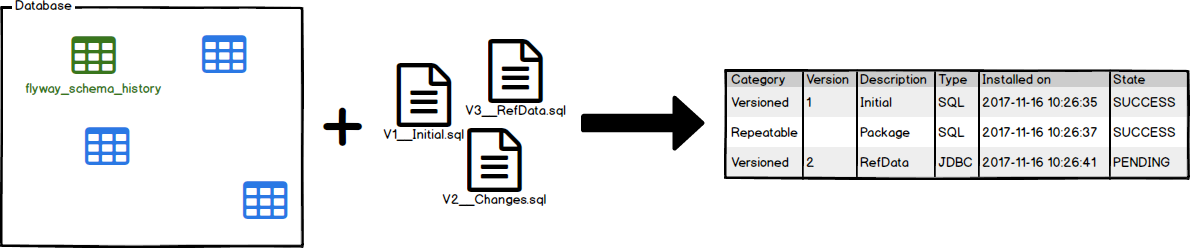
\includegraphics[width=0.8\textwidth]{./chapters/intro_flyway/images/command-info}
	\caption[Flyway Info - Source: \cite{FlywayGetStarted}]{Flyway Info}
	\label{fig:command-info}
\end{figure}

\todo{write all titles big or small?}
\textbf{clean}\\
With \texttt{flyway clean}, one can drop all objects, like tables, views and triggers, in the configured schemas. It serves as a reset but is dangerous in a production environment.

\textbf{Validate}\\
To ensure that all migrations are applied correctly,  \texttt{flyway validate} is the choice command. The validation checks if the migration locally has the same checksum as the migration executed in the database.
There is a possibility to apply custom validation rules. Because in a productive environment, there will be hotfixes, deleted migrations and other changes that break the default validation conventions. Custom rules are only available in the teams edition.

\textbf{Repair}\\
However, if something is broken, the repair command can repair the database, especially the checksum. For example, when a database migration fails, the migration is marked as failed in the schema history table (\textit{flyway\_schema\_history}). However, if a database supports \gls{DDL} transactions (like PostgreSQL), the failed migration is rolled back automatically, and nothing is recorded in the schema history table. Nevertheless, if the database does not support DDL transactions (e.g. Oracle Database, MySQL, MariaDB), you have two options to repair the database and remove the failed entries:

\begin{enumerate}
	\item Run \texttt{flyway repair}\\
	\item One uses the flyway callback functions. One could use the \textit{afterMigrateError} and add a SQL-script to this callback, which deletes the failed migration entry in the \textit{flyway\_schema\_history} table.
	
	\begin{lstlisting}[language=SQL]
		DELETE IGNORE FROM flyway_schema_history WHERE success=0;
	\end{lstlisting}
\end{enumerate}


\textbf{Undo}\\
To undo the most recent migration applied to the database, run \texttt{flyway undo}. The undo command can be repeated until the database is converted back to version 1. Undo assumes that the previously applied migration succeeded and now should be undone. If the previously applied migration fails, repair the migrations before applying the undo command. The undo command is a Teams Edition feature only.

\textbf{Baseline}\\
This command makes the current database the baseline for the future. This will cause the migrate command to ignore all migrations up to the actual version. This can be useful to reduce the overhead if many old migrations scripts exist that will not be used again.

\section{Installation and Setup}
\marginpar{Different usages of Flyway \cite{FlywayGetStarted}}%
Flyway can be used with the following programs or tools.

\begin{minipage}[t]{0.5\textwidth}
\textbf{Flyway Clients}

\begin{itemize}
	\item \Gls{CLI}
	\item \gls{JAVAg} \acrshort{API}
	\item Maven
	\item Gradle
\end{itemize}
\end{minipage}
\begin{minipage}[t]{0.5\textwidth}
	\textbf{Third Party Plugins}
	\begin{itemize}
		\item Jenkins
		\item IntelliJ IDEA
		\item NPM
		\item Play
		\item Spring Boot
		\item etc.
	\end{itemize}
\end{minipage}
\vspace{0.3cm}

\marginpar{CLI installation}%
Download the latest version of the \href{https://flywaydb.org/download/community}{Flyway Cummunity Edition} and extract the downloaded file. To execute the flyway commands, one need a java installation.
Once extracted, the file becomes a directory with the following structure:

\begin{figure}[H]
    \centering
    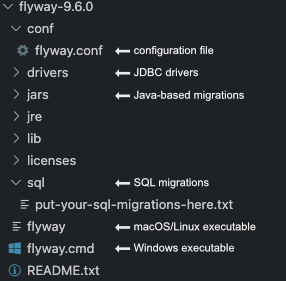
\includegraphics[width=0.4\textwidth]{./chapters/intro_flyway/images/flyway_folder_structure}
   \caption[Flyway folder structure - Source: Own illustration]{Flyway folder structure}
    \label{fig:flyway_folder_structure}
\end{figure}


\marginpar{Configuration}%
To connect to a running database, add the relevant information to \textit{conf/flyway.conf}.
In our minimal example this could be:

\begin{lstlisting}[caption=Minimal configuration]
flyway.url=jdbc:postgresql://localhost:5432/pagila
flyway.user=postgres
flyway.password=password
\end{lstlisting}

\todo{footnote or rather add to bibliography and cite?}
This is just a minimal configuration, but there are many more additional parameters that can be set \footnote{\url{https://flywaydb.org/documentation/configuration/parameters/}}.


\marginpar{Workaround Mac OS}%
To make the flayway command know on MacOS:
\begin{lstlisting}[caption=Minimal configuration]
export PATH=$PATH:/Users/marco/Documents/DB-Seminar/flyway-9.8.1
\end{lstlisting}
Running a flyway command for the first time, the error message \textit{„java“ kann nicht geöffnet werden, da der Entwickler nicht verifiziert werden kann.} occurs. Go to Security in settings and allow the java instance to run.

\newpage

% !TeX spellcheck = en

\chapter{Introduction to Liquibase}
\section{Overview}
Provide a detailed overview of the Liquibase tool.

\marginpar{Community}%
Stars on GitHub: 3'600 (27. December 2022)\\
Tags on StackOverflow: 3,530 (27. December 2022)\\

\section{Functionality with Simplistic Example}
Explain how the Liquibase tool works and provide a simplistic example to demonstrate.




\todo{updateSQL}
Die Funktion updateSQL von LiquiBase
Ermöglicht, die anstehende Migration zunächst als SQL-Befehle auszugeben, z.B. zu Review- Zwecken.
Ist bei Flyway nicht relevant, da Plain-SQL-Skripte verwendet werden


\newpage

% !TeX spellcheck = en

\chapter{Database Change Scenarios}
This section shows how to handle the predefined scenarios for the given change management tool. This includes following scenarios: 

\begin{itemize}
	\item Rename an attribute.
	\item Add an attribute and set the value as a constant.
	\item Delete an attribute.
	\item Change an attribute type and add an SQL script to fill it from existing values.
	\item Rename a table and change a related view which uses this table.
\end{itemize}

The changes were applied to an existing database Pagila \cite{Hillyer}. Each first two migrations are to setup the database, first the create the schema and second to insert the specific data.

\section{Flyway Scenarios}

\subsection{Using CLI}
\marginpar{Setup \cite{FlywayGetStarted}}%
To create a first migration, add a database change as sql file into the sql directory (see \autoref{fig:flyway_folder_structure}). 
The scripts \texttt{V1\_\_create\_db.sql} and \texttt{V2\_\_insert\_pagila\_data.sql} set up the pagila database as illustrated in \autoref{fig:flyway_empty_db}. When running  \texttt{flyway migrate}, flyway wants to adapt the schema history table. But as this table does not exist, it will create a new one instead.


 

\begin{figure}[H]
	\centering
	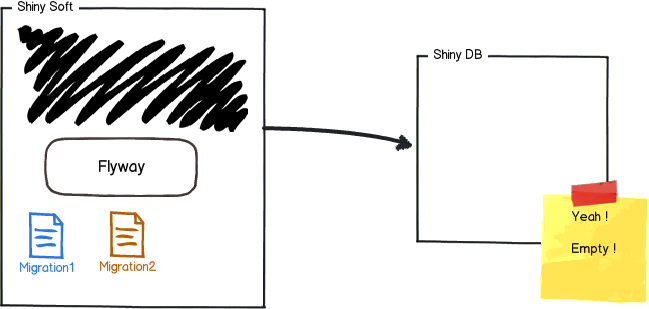
\includegraphics[width=0.45\textwidth]{./chapters/scenarios/images/EmptyDb}
	\caption[Flyway empty database - Source: \cite{FlywayGetStarted}]{Flyway empty database}
	 \label{fig:flyway_empty_db}
\end{figure}
Now the table \textit{flyway\_schema\_history} has been created via the first flyway migration. This metadata table holds various information regarding the database migrations and their history. After this initialization, flyway runs the migration scripts in the sql directory according on their version number subsequently. 
BASELINE MODEL! To start with a baseline

\begin{figure}[H]
	\centering
	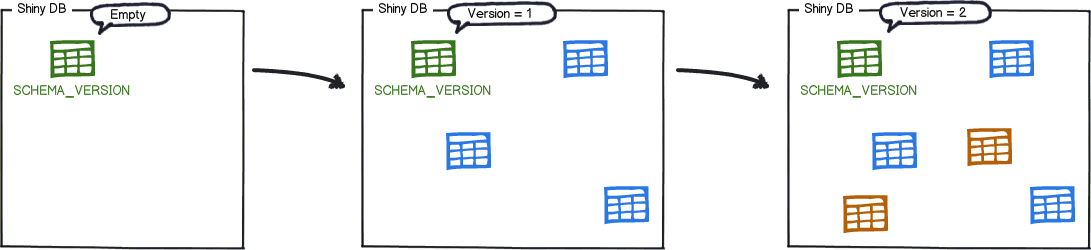
\includegraphics[width=0.85\textwidth]{./chapters/scenarios/images/Migration-1-2}
	\caption[Flyway first migrations - Source: \cite{FlywayGetStarted}]{Flyway first migrations}
	\label{fig:Migration-1-2}
\end{figure}


\marginpar{Rename an attribute}%
The first change specific migration is in the sql migration script\\ \texttt{V3\_\_rename\_attribute.sql}:
\begin{lstlisting}[language=SQL]
ALTER TABLE customer RENAME COLUMN email TO private_email;
\end{lstlisting}
After just adding the script to de sql directory, flyway already knows the change and stores it into the meta data table. With \texttt{flyway info} the migration status can be asked:

\begin{figure}[H]
	\centering
	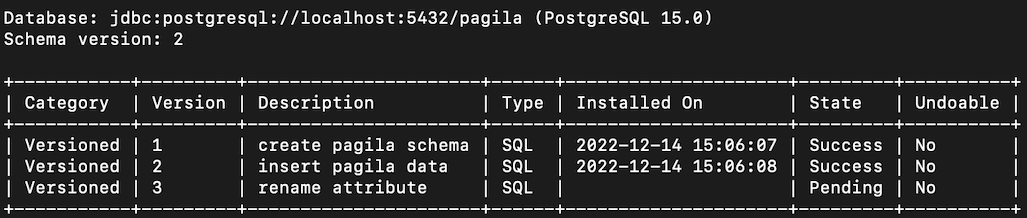
\includegraphics[width=0.95\textwidth]{./chapters/scenarios/images/flyway_metadata_v2}
	\caption[Flyway meta data table - Source: Own illustration]{Flyway meta data table}
	% \label{fig:bsp_chapter:example_figure}
\end{figure}
In order to perform the migration effectively, the command \texttt{flyway migrate} is applied.



\marginpar{Add an\\ attribute}%
To apply the second migration the following script is applied in V3.
\begin{lstlisting}[language=SQL]
ALTER TABLE customer ADD COLUMN gender VARCHAR(50);

UPDATE customer
SET gender = 'undefined';
\end{lstlisting}
Flyway generates a checksum for every applied migration. This checksum is used to track if a file was changes after its applied migration. If such a change occurs, a new migration will cause an error and asks to either revert the change or to run \texttt{flyway repair} to update the schema history.
If a developer would change the default value of gender from \textit{undefined} to \textit{undef} and run a new migration, it would fail. To fix this run \texttt{flyway repair}. Even the environment is now fixed, the change gender equals \textit{undef} is not applied and still \textit{undefined}.


\marginpar{Delete an\\ attribute}%

\begin{lstlisting}[language=SQL]
ALTER TABLE customer
DROP COLUMN gender;
\end{lstlisting}
\todo{chan delete be undoable? Without extra effort.
	How can I undo the deletion? Requires flyway teams.
}

\marginpar{Change an attribute typ}%
To change an attribute type the migration in the file \texttt{V6\_\_change\_attribute\_type.sql} was applied with flyway migrate:
\begin{lstlisting}[language=SQL]
ALTER TABLE customer
ALTER COLUMN private_email TYPE VARCHAR(100) USING private_email::varchar;
\end{lstlisting}


\marginpar{Rename a table and change related view}%
The last migration is to change a related view after renaming a table\\
\texttt{V7\_\_change\_attribute\_type.sql} was applied with flyway migrate:
\begin{lstlisting}[language=SQL]
ALTER TABLE customer RENAME TO clients;
	
	
CREATE OR REPLACE VIEW customer_list AS
SELECT cl.customer_id AS id,
	(cl.first_name || ' '::text) || cl.last_name AS name,
	a.address,
	a.postal_code AS "zip code",
	a.phone,
	city.city,
	country.country,
	CASE
		WHEN cl.activebool THEN 'active'::text
		ELSE ''::text
	END AS notes,
	cl.store_id AS sid
FROM clients cl
JOIN address a ON cl.address_id = a.address_id
JOIN city ON a.city_id = city.city_id
JOIN country ON city.country_id = country.country_id;
\end{lstlisting}

After this last migration the flyway schema history looks like the following:
\begin{figure}[H]
	\centering
	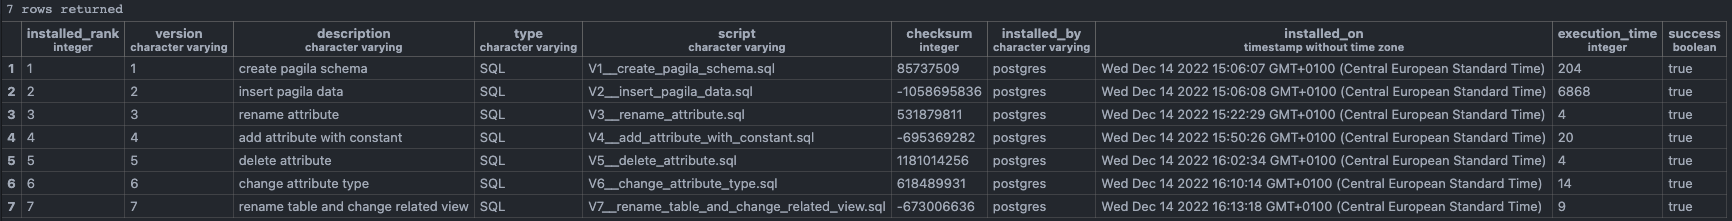
\includegraphics[width=1.1\textwidth]{./chapters/scenarios/images/flyway_schema_history}
	\caption[Flyway Schema History - Source: Own illustration]{Flyway Schema History}
	% \label{fig:bsp_chapter:example_figure}
\end{figure}
For every migration the date inclusive time, the script or the user that applied the script is stored.

\marginpar{Failed migration \cite{Lukonin2017}}%
Flyway automatically wraps every migration script in a transaction, which allows for automatic rollback in case of an error. If your database supports DDL transactions (such as PostgreSQL), the entire migration script will be rolled back automatically. However, if you are using SQL Server, the DDL queries will be committed automatically, so you will need to create manual rollback scripts or use idempotent scripts to roll back the changes. If your migration script does not contain DDL commands, it will generally be automatically rolled back by most database engines in case of an error.\\
To make the rollback process easier, Flyway supports rollback scripts, which can be created for every versioned migration file using the naming convention \textit{U\#\#\#\_\_text.sql}. If a migration fails, Flyway will automatically run the corresponding rollback script. The UNDO command (see \autoref{flyway_features}) can also be used to manually trigger a rollback, which will roll back the latest migration by default. Alternatively, taking a snapshot of the database before release and restoring it if any migration goes wrong is the cleanest approach, but may not always be feasible. It is important to have a well-designed rollback strategy in place, which may involve creating proper rollback scripts and using idempotent migrations to make the process easier.

\subsection{Usage with Java API}
\marginpar{JavaAPI}%
TODO\\



\newpage
\section{Liquibase Scenarios}



\newpage

% !TeX spellcheck = en

\chapter{Flyway vs. Liquibase}

In this section we aim to compare Flyway and Liquibase according to sources \cite{Parsick2018}, \cite{Kaps2016}, \cite{LiquibaseVSFlyway}, \cite{Zylinski2022} and our personal experience gained during this seminar.\\

\section{Comparison}
\marginpar{Commonalities}%
First of all, both tools use a migration-based approach for changes and are open source (Apache v2  \footnote{\url{https://github.com/flyway/flyway/blob/main/LICENSE.txt}} \footnote{\url{https://github.com/liquibase/liquibase/blob/master/LICENSE.txt}}) and in our opinion very easy to use and light-weighted.
Both offer things like repeatable migrations, checksum validation, placeholder replacement and are cluster-safe.
In addition, both tools provide the common interfaces such as CLI, Java API, Maven, Ant, Spring etc.
The list of supported databases is largely the same for both systems, with only minor variations in supported versions or drivers. In general, there are no significant differences in terms of database support between the two systems.


\marginpar{Popularity}%
\textbf{Community}\\
Both have a similarly large community according to the refrences Github stars (Flyway: 6900, Liquibase: 3600) or tags on Stack overflow (Flyway: 2118, Liquibase 3530). 

The search queries on Google also show that both receive a similar number of requests, but Liquibase is slightly ahead. The increase in searches in December 2021 is due to improvements in data collection. 
\begin{figure}[H]
	\centering
	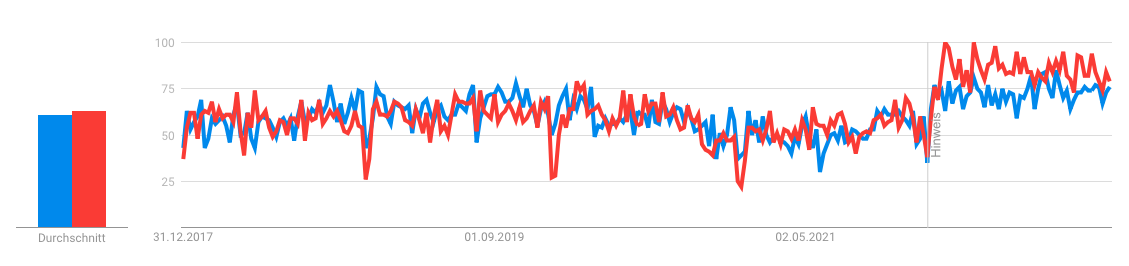
\includegraphics[width=0.9\textwidth]{./chapters/flyway_vs_liquibase/images/flyway_liquibase_search_history}
	\caption[Google Search interest over time - Source: Google Trends]{Google Search interest over time - Source: \url{trends.google.com}}
	% \label{fig:bsp_chapter:example_figure}
\end{figure}


\textbf{Integration into existing projects}\\
In order to be able to integrate existing projects in with flyway, one has to create a manual dump (DDL) of the production database as version 1 script, first clean and empty all other databases and migrate to version 1. Alternatively, you can manually bring the other databases to the state of the production database and set the state as version 1 using the baseline command.\\
On the other hand, in Liquibase it works the following. To tag the state of the production database as version 1, use the \package{generateChangelog} command. To compare the production database with other environments, use the diff command and generate changelogs for any differences. You can mark the generated changelogs as "already run" or exclude them from future runs as needed.\\
LiquiBase integration is highly promising due to the clever combination of its powerful functions. The integration of flyway seems more like a workaround solution.\\

\textbf{Functionalities}\\
In the table x you can see that Liquibase has more functionalities in the ratio 16/9. 



\begin{table}[H]
	\centering
	\ra{1.2}
	\begin{tabularx}{10cm}{X c c}
		\toprule
		Function  & 	Flyway & Liquibase \\
		\midrule
		Migration & +++ & +++ \\
		& \package{migrate} & \package{update} \\ \hline
		
		Rollback & - & ++ \\
		& \package{undo} (pro version) & \package{rollback} \\ \hline
		
		Clear schema & + & + \\
		& \package{clean} & \package{dropAll} \\ \hline
		
		Documentation & + & ++ \\
		& \package{info} & \package{DBDoc} \\ \hline
		
		Comparison & - & ++ \\
		&  & \package{Diff} \\ \hline
		
		Validation & + & - \\
		& \package{validate} & \\ \hline
		
		Initialization & + & - \\
		& \package{baseline} & \\ \hline
		
		Maintenance & + & + \\
		& \package{repair} & \package{clearChecksums} \\ \hline
		
		Callbacks & + & -\\
		& & \\ \hline
		
		Preconditions & - & + \\
		& & \\ \hline
		
		Context & - & ++ \\ 
		& & \\ \hline
		
		Refactoring & - & ++ \\
		& & \\
		\bottomrule
	\end{tabularx}
	\caption{Functionalities Flyway vs. Liquibase - Based on \cite{Zylinski2022}}
	\label{tab:functionalities_flyway_liquibase}
\end{table}





\begin{table}[H]
	\centering
		    \begin{tabular}{|l|p{.45\textwidth}|p{.45\textwidth}|}
		    \hline
			 & Liquibase & Flyway\\ \hline
			 \begin{turn}{-90}Advantages\end{turn} &
			\begin{itemize}
				\item More functionalities such as diff generation (compare two databases), Rollbacks, or monitoring and dashbording possibilities
				\item Apply the same scripts to different database vendors
				\item Integration of existing databases is more promising
				\item Work with NoSQL and relational database types
				\item DDL abstraction DSL (todo: ?)
				\item More flexible when it comes to deployment (selective deployments and rollbacks)
			\end{itemize} & \begin{itemize}
				\item Very easy and intuitive to use
				\item Direct use of SQL files
				\item Multiple schema support
				\item Clean existing schema
			\end{itemize}\\ \hline
		
	 \begin{turn}{-90}Disadvantages\end{turn} &
		\begin{itemize}
			\item Steeper learning curve and more complicated 
			\item No direct support for Java migrations
		\end{itemize} & \begin{itemize}
			\item Important features like Undo or Dry-Run are not included in the free version 
			\item No support for older Java version such as Java 6 \& 7 (enterprise only)
			\item Versioning system with linear naming convention makes it hard to manage the order of changes
		\end{itemize}\\ \hline
		\end{tabular}
	\caption{Flyway vs Liquibase comparison - Based on \cite{Parsick2018, Kaps2016}}
	\label{tab:flyway_liquivase_conparison}
\end{table}

\newpage
\section{When to use which?}

\marginpar{Question for Selection\\ \cite{Zylinski2022}, \cite{LiquibaseVSFlyway}}%
Even though both provide the basic change management functions perfectly,
there are specific differences in their use. With the following questions the selection can be summed up:

\textit{Does the project use a specific database that only one tool supports?}\\
At the beginning, the framework conditions should be checked whether a certain tool can be used at all. For example, if you also want to integrate NoSQL databases, only Liquibase and not Flyway offers this.

\textit{Do you want to continue using your previous SQL scripts 1:1?}\\
With Flyway, SQL scripts can be integrated directly. Only the name of the script would have to be adapted. When using Liquibase, the changelog files would have to be rewritten again.

\textit{Is it possible to do without rollbacks? (e.g. through clever forward migrations)}\\
Since Flyway does not offer rollbacks in the free version, the choice would fall on Liquibase. However, if you can work around this, there is no disadvantage to using Flyway in this regard.

\textit{Do you need German support?}\\
Since Liquibase is an American company, it provides information in English only. Flyway offers support in several languages and also in German.

\textit{Do you want to have your test data managed as well?}\\
\todo{..}

\textit{Do you want to support diverse DBMS?}\\
Liquibase allows you to use XML, YAML, or JSON to define your database changes, providing an abstraction layer that makes it better suited for use in software products that may be installed in different environments with different underlying database technologies. With Flyway one writes the migrations directly in the SQL language of the used database, therefore with flyway you would have to rewrite the scripts for another database. Probably a lot can be taken over, but there is no guarantee what ends in a manual additional effort.

\textit{Are there many different environments with different database schema requirements?}\\
If this is a requirement, Liquibase is the tool of choice because one can selectively deploy changes as needed to different environments. 
Liquibase offers support for updating and managing the same schema across multiple database vendors \& platforms using the same changelog file.
In addition there is support to easily add new changes and reorder them without running into filename conflicts

\textit{How large is the development team?}\\
\todo{..}


\newpage
%!TeX spellcheck = en

\chapter{Results}

\section{Discussion}
\marginpar{Change Management}%
Key takeaways from Piairo et al. 2018 \cite{Piairo2018}:

\begin{itemize}
	\item Databases, although different from applications, can and should be included in the same development process as applications. We call this database shift left.
	\item When all database changes are described with scripts, source control can be applied, and the database development process can include continuous integration and continuous delivery activities, namely taking part in the deployment pipeline.
	\item Automation is the special ingredient that powers up the deployment pipeline making it repeatable, reliable and fast, reducing fear of database changes.
	\item Migrations-based and state-based are two different approaches to describing a database change. Independently of choice, small batches are always a good choice.
	\item The deployment pipeline is a technical and cultural tool where DevOps values and practices should be reflected according to the needs of each organisation.    
\end{itemize}

\marginpar{Flyway vs Liquibase}%
Flyway and Liquibase are open-source database change management tools that help organisations track, version, and deploy changes to their databases. Both tools support various database platforms and offer version control, change tracking, and rollback capabilities.

One key difference between the two tools is how changes are defined. Flyway uses SQL scripts to define changes, while Liquibase allows changes to be defined using XML, YAML, or JSON files. This means that Liquibase provides an abstraction layer that can make it easier to manage changes in environments where the underlying database technology may vary.

Another difference is how changes are applied. Flyway applies changes in a linear, version-based sequence, while Liquibase allows for more flexible change ordering and dependencies. This can make Liquibase better suited for complex change management scenarios but may also make it more challenging for simple deployments.

Overall, the choice between Flyway and Liquibase will depend on an organisation's specific needs and constraints. However, both tools are widely used and have strong communities of users and contributors, so either tool may be a good fit for a given project.

\section{Lesson learned}
The project teaches about the importance of database change management and the integration of data ops into the workflows of database management. Learning the state-of-the-art methods and exploring the developed tools such as Liquibase and Flyway is refreshing. We learned how easily Liquibase and Flyway work and how to use them to manage a database and gained insights on the best practices by using the tools ourselves. Database schema management is for more than just big teams with massive databases. Even small teams can benefit from the vast features and the version control it allows.










% %!TeX spellcheck = en

\chapter{Outlook}
This section aims to provide an outlook on further tool / research and additional material.

%!TeX spellcheck = en

\chapter{Possible MSE Data Engineering Exercise}

\section{Task}

\section{Sample Solution}




% Bibliography
\cleardoublepage
\chapter*{Bibliography}
\addcontentsline{toc}{chapter}{Bibliography}
\printbibliography[heading=none]


% Appendix

\glsaddall
\printglossary

% Appendix
\appendix
\appendixpage
\noappendicestocpagenum
\addappheadtotoc

\markleft{\glossaryname}
%\printnoidxglossary[type=\acronymtype]
\printnoidxglossary[nonumberlist]

\listoffigures
\listoftables


%\cleardoublepage
%\chapter{Task}
%\newpage
%\begin{figure}[H]
%	\includepdf[pages=1]{appendices/Aufgabenstellung/..}
%\end{figure}
%
%\newpage
%\begin{figure}[H]
%	\includepdf[pages=2]{appendices/Aufgabenstellung/..}
%\end{figure}
%
%
%\cleardoublepage
%\chapter{Time schedule}
%\newpage
%\begin{figure}[H]
%	\includepdf[landscape]{appendices/..}
%\end{figure}






%% !TeX spellcheck = en_US

\chapter{Beispiel}

\marginpar{Goal of this chapter}% This comment after \marginpar is needed so there is no space before the paragraph.
This chapter is to demonstrate some of the capabilities of this \LaTeX{} template.
Please take a good look at this chapter and try to follow the guidelines.

\section{Equations}
\subsection{some equations}
\marginpar{Equations}%
%\glspl{equation}\index{Equation} can easily be written using the \emph{\gls{equation}}
environment. Inline equations are inserted with $\sqrt{-1} = i $. Equations can
also be labeled, so it is possible to reference them. This should be done for
all important equations.

\begin{equation}
    x^2 + y^2 = 1
    \label{equ:bsp_chapter:example_equation}
\end{equation}

\begin{lstlisting}[language=C,label=bsp,caption=bsp]
	# include "hoi.h"
	int i = 0;
\end{lstlisting}

\begin{lstlisting}[label=bsp,caption=bsp]
	import cv2
	import numpy as np
	from pyzbar.pyzbar import decode
\end{lstlisting}

%\lstinputlisting[language=Python, firstline=60, lastline=67]{appendices/Quellencodes/cv/cv.py}

There are several environments for multi line equations. A very useful one
is \emph{align}, see equation %\eqref{equ:bsp_chapter:example_align}.

\begin{align}
    \oint \vec{E} \cdot d \vec{A} & = \frac{q}{\epsilon_0}  \\
    \oint \vec{B} \cdot d \vec{A} & = 0                     \\
    \oint \vec{E} \cdot d \vec{s} & = - \frac{d \Phi_B}{dt}
    \label{equ:bsp_chapter:example_align}
\end{align}

\begin{equation}
    \begin{split}
        W_{V12} &= 4 \cdot 10^5\ Pa \cdot 4\ m^3 \cdot \ln(\frac{4\ bar}{4\ bar}) \\
        W_{V12} &\approx 4\ J
    \end{split}
\end{equation}

\marginpar{Figures and Tables}%
Images\index{Image} are always inserted inside a \emph{figure}
environment. If possible, it is advisable to use \texttt{[tb]} as position.
Always remember to add a caption and a label, so you can reference the image
like this: \autoref{fig:bsp_chapter:example_figure}. If possible, images should be
inserted as vector graphics, e.g. \texttt{eps} or \texttt{pdf} - or even drawn
manually in TikZ.

\begin{figure}[t]
    \centering
    
\includegraphics[width=2cm]{chapters/Beispiel/images/thumbs_up.jpg}
    \caption{An example image}
    \label{fig:bsp_chapter:example_figure}
\end{figure}

Tables \index{Table} can be used quite similarly. They are inserted inside a \emph{table} \index{Table!tabular}
environment, as shown in \autoref{tab:bsp_chapter:example_table}.

\begin{table}[t]
    \centering
    \begin{tabular}{lcrp{4cm}} \toprule
        some          & text      & is shown & here  \\ \midrule
        there is more & text here & and here & cool. \\
        and           & even      & more     & here. \\ \bottomrule
    \end{tabular}
    \caption{A sample table}
    \label{tab:bsp_chapter:example_table}
\end{table}

Another useful tool is the \emph{tabularx} environment. \index{Table!tabularx}
It lets the user specify the total width of the table, instead of each column.
An example is shown in \autoref{tab:bsp_chapter:example_tabularx}.

\begin{table}[t]
    \centering
    \begin{tabularx}{0.9\linewidth}{lXX} \toprule
        some          & text      & is shown here \\ \midrule
        there is more & text here & and here.     \\
        and           & even      & more here.    \\ \bottomrule
    \end{tabularx}
    \caption{Tabularx example}
    \label{tab:bsp_chapter:example_tabularx}
\end{table}

\begin{table}[H]
    \centering
    \begin{tabular}[H]{llp{5cm}}
        Augmenter      & Parameter          & Beschreibung                                                                                                           \\ \hline
                       &                    &                                                                                                                        \\
        Rotate         & $\pm$ 5\textdegree & Bilder werden zufällag bis zu fünf Grad nach links oder rechts um den Bildmittelpunkt gedreht.                         \\
                       &                    &                                                                                                                        \\
        LinearContrast & $\alpha$ = 0.5-1.5 & Erhöht oder verringert Kontrast der Bilder um den Faktor Alpha der pro Bild zufällig aus einem Intervall gewählt wird. \\
    \end{tabular}
    \caption{Beispieltabelle}
    \label{}
\end{table}

Please read the documentation of the
\emph{booktabs}\footnote{\url{http://www.ctan.org/pkg/booktabs}}
package to find information on how to create good tables.
Always remember the first two guidelines and try also to stick to the other three:
\begin{enumerate}
    \item Never, ever use vertical rules.
    \item Never use double rules.
    \item Put the units in the column heading (not in the body of the table).
    \item Always precede a decimal point by a digit; thus $0.1$ \emph{not} just $.1$.
    \item Do not use \enquote{ditto} signs to repeate a value. In many circumstances a blank will serve just as well. If it won't, then repeat the value.
\end{enumerate}

\marginpar{Paragraphs}%
Note that each paragraph is ended with an empty line.
\emph{Never} use \verb|\\| to end paragraphs -- this is a new line, not a new paragraph.
Also try to keep your source code clean: about 80 characters per line.
Using source control makes your life much easier

\marginpar{Quotes}%
Quotes can easily be made using the \enquote{csquotes} package.
Citing text passages is easily done: \textquote[me][!]{First argument: citation,
    second argument: terminal punctuation} Whole block quotes are also easily
possible.

\blockquote{Formal requirements in academic writing frequently demand that
    quotations be embedded in the text if they are short but set oV as a distinct
    and typically indented paragraph, a so-called block quotation, if they are
    longer than a certain number of lines or words. In the latter case no quotation
    marks are inserted.}

\marginpar{SI Units}%
Any numbers and units should by typed using the siunitx package.
Numbers are written as \num{1234} \num{3.45e-5} \numlist{1;2;4} \numrange{4}{30} \ang{10} \ang{5;3;2}.
Units are written with \si{\kilo\gram\meter\per\square\second} or \SI{14}{\farad\tothe{4}}.
Of course also possible is \SIlist{10;40;12}{\meter} or \SIrange{-40}{+125}{\degreeCelsius}
Almost every unit you could possibly think of is implemented!

\marginpar{Bibliography}%
The bibliography is created using \emph{Bibtex}. The
standard format is set to \texttt{ieeetr}, which is the IEEE Standard. There
are example entries for different types of  in the separate bibliography file
%\cite{article} \cite{book} \cite{booklet} \cite{conference} \cite{inbook}
\cite{incollection} \cite{manual} \\
%\cite{phdthesis} \cite{proceedings} \cite{techreport} \cite{unpublished}.


Cite a page: \cite[p. 435]{incollection} \\
Cite several pages: \cite[pp. 436-440]{incollection}\\

\marginpar{Index \& Glossary}%
All glossary entries are made in the separate file \texttt{glossary.tex}.
%They can then be used with \gls{equation}.
Acronyms are defined as shown there and used similarly.
The first time, it will be \emph{\gls{svm}}.
The second time: \emph{\gls{svm}}.
The glossary has to be created manually by invoking \texttt{makeindex -s doku.ist -t doku.glg -o doku.gls doku.glo}.
The index is simply created by using \texttt{index\{text\}}. It is generated automatically.

\subsection{Listings}
Listings are created by the \texttt{lstlistings} package.

\todo{This is a simple ToDo note}

\todonote{This is a small note}
\citationneeded

\hlc[pink]{hello}

\subsection{Algoruthms}
\begin{algorithm}[H]
    \SetAlgoLined
    \KwResult{Write here the result }
    initialization\;
    \While{While condition}{
        instructions\;
        \eIf{condition}{
            instructions1\;
            instructions2\;
        }{
            instructions3\;
        }
    }
    \caption{How to write algorithms}
\end{algorithm}


\subsection{Images}

\begin{figure}[H]
    \begin{subfigure}{0.3\textwidth}
        \centering
        
\includegraphics[width=0.5\textwidth]{chapters/Beispiel/images/thumbs_up.jpg}
        \caption[blabla\quad - Bildquelle: \cite{}]{bla bla}
        \label{}
    \end{subfigure}%
    \begin{subfigure}{0.7\textwidth}
        \centering
        
\includegraphics[width=0.5\textwidth]{chapters/Beispiel/images/thumbs_up.jpg}
        \caption[blabla2 \quad - Bildquelle: \cite{hsv1}]{bla bla2}
        \label{f}
    \end{subfigure}%
    \caption[bla bla bla bla]{bla bla bla bla}
\end{figure}

%% !TeX spellcheck = de_DE

\chapter{Cheat Sheet}


\marginpar{Funktion}%
Nachdem das Kamerabild eingelesen worden ist, sollen die entsprechenden Objekte gefunden werden. Mit diesen Informationen soll dann der Abstand zum Objekt ermittelt werden und via serielle Schnittstelle an die Fahrplattform übertragen werden.




\section{Listing}
\begin{enumerate}[label=(\alph*)]
	\item Pixelwert wird unterdrückt (Wert = 0), da es sich nicht um das Maximum in die Gradientenrichtung $- \pi$ handelt
	\item Bildet das lokale Maximum in Gradientenrichtung $\frac{3 \pi}{4}$, Pixelwert wird nicht verändert
	\item Bildet auch das lokale Maximum in Gradientenrichtung, Pixelwert wird nicht verändert
\end{enumerate}


\section{Cite and reference and format}

Reference: \autoref{fig:hsv2} \\


Cite: \cite{xlinuxai}\\


Package: \package{TFLite Model Maker} \\

Footnote: \footnote{{https://www.tensorflow.org/lite/guide/model\_maker}}

\section{Images}

\begin{figure}[H]
	\centering
	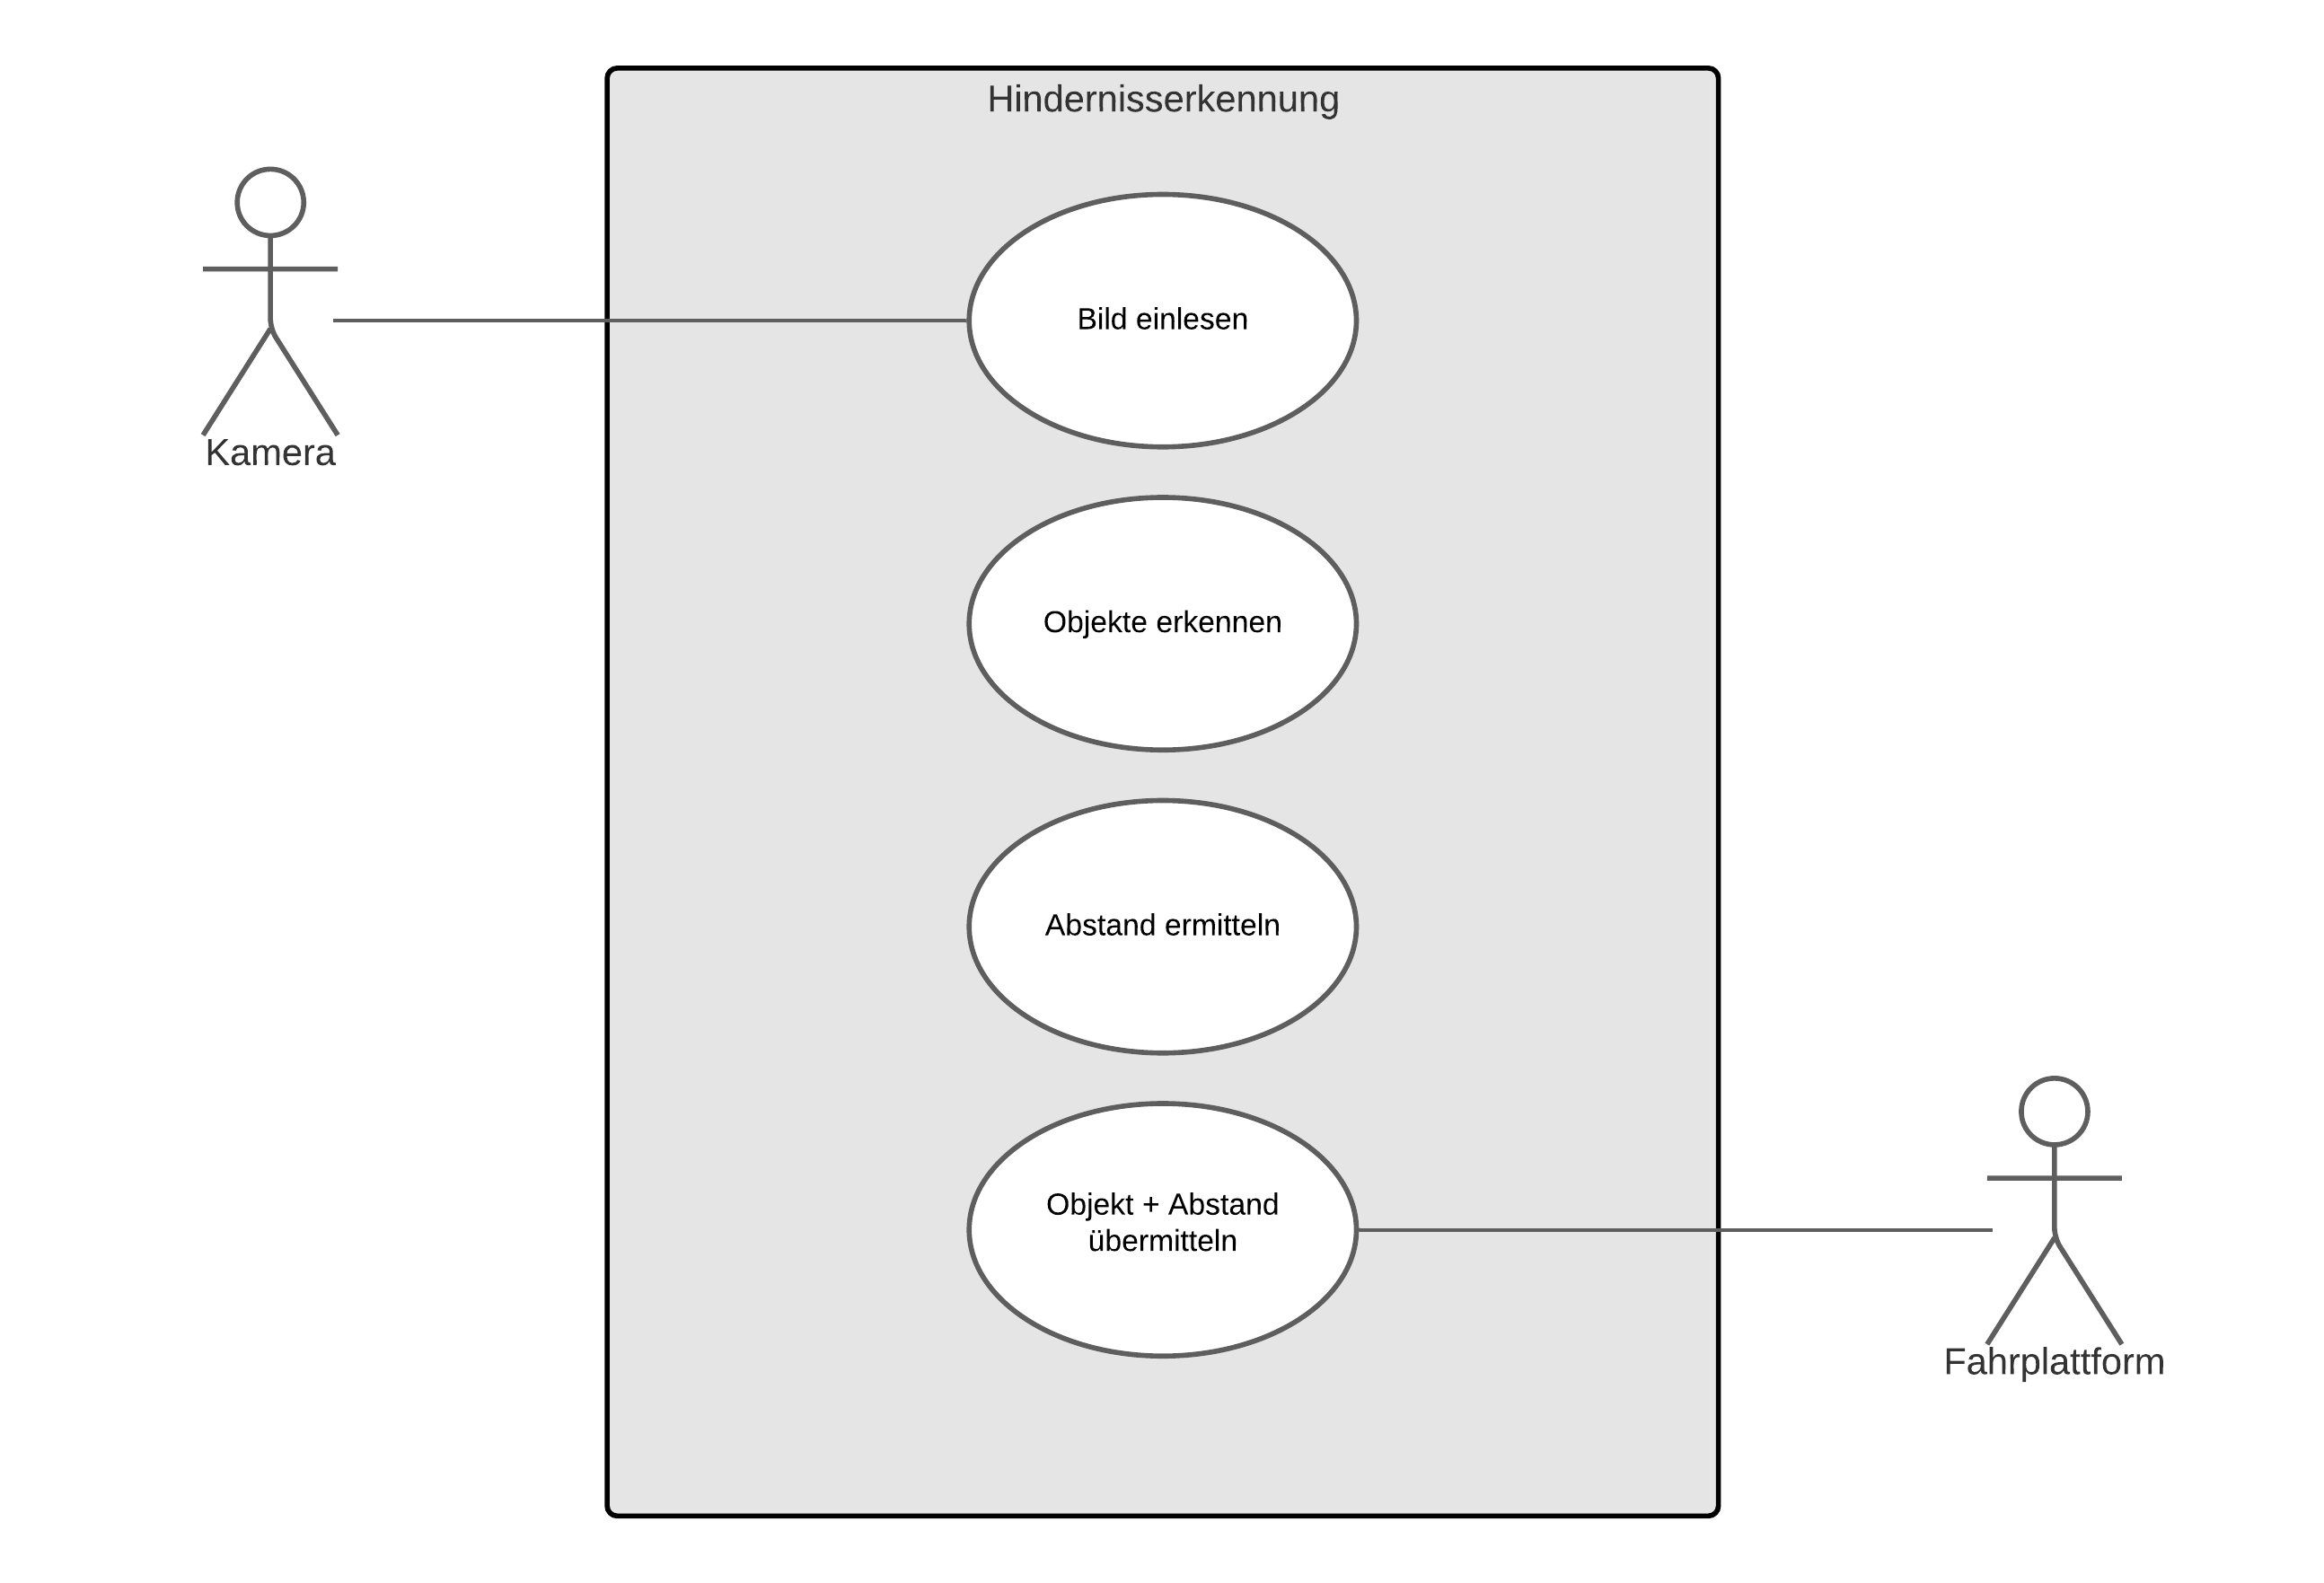
\includegraphics[width=0.35\textwidth]{chapters/cheatsheet/images/UseCaseNeu.png}
	\caption[Use Case Diagramm - Eigene Darstellung]{Use Case Diagramm}
	\label{fig:usecase1}
\end{figure}

\begin{figure}[H]
	\begin{subfigure}{0.3\textwidth}	
		\centering
		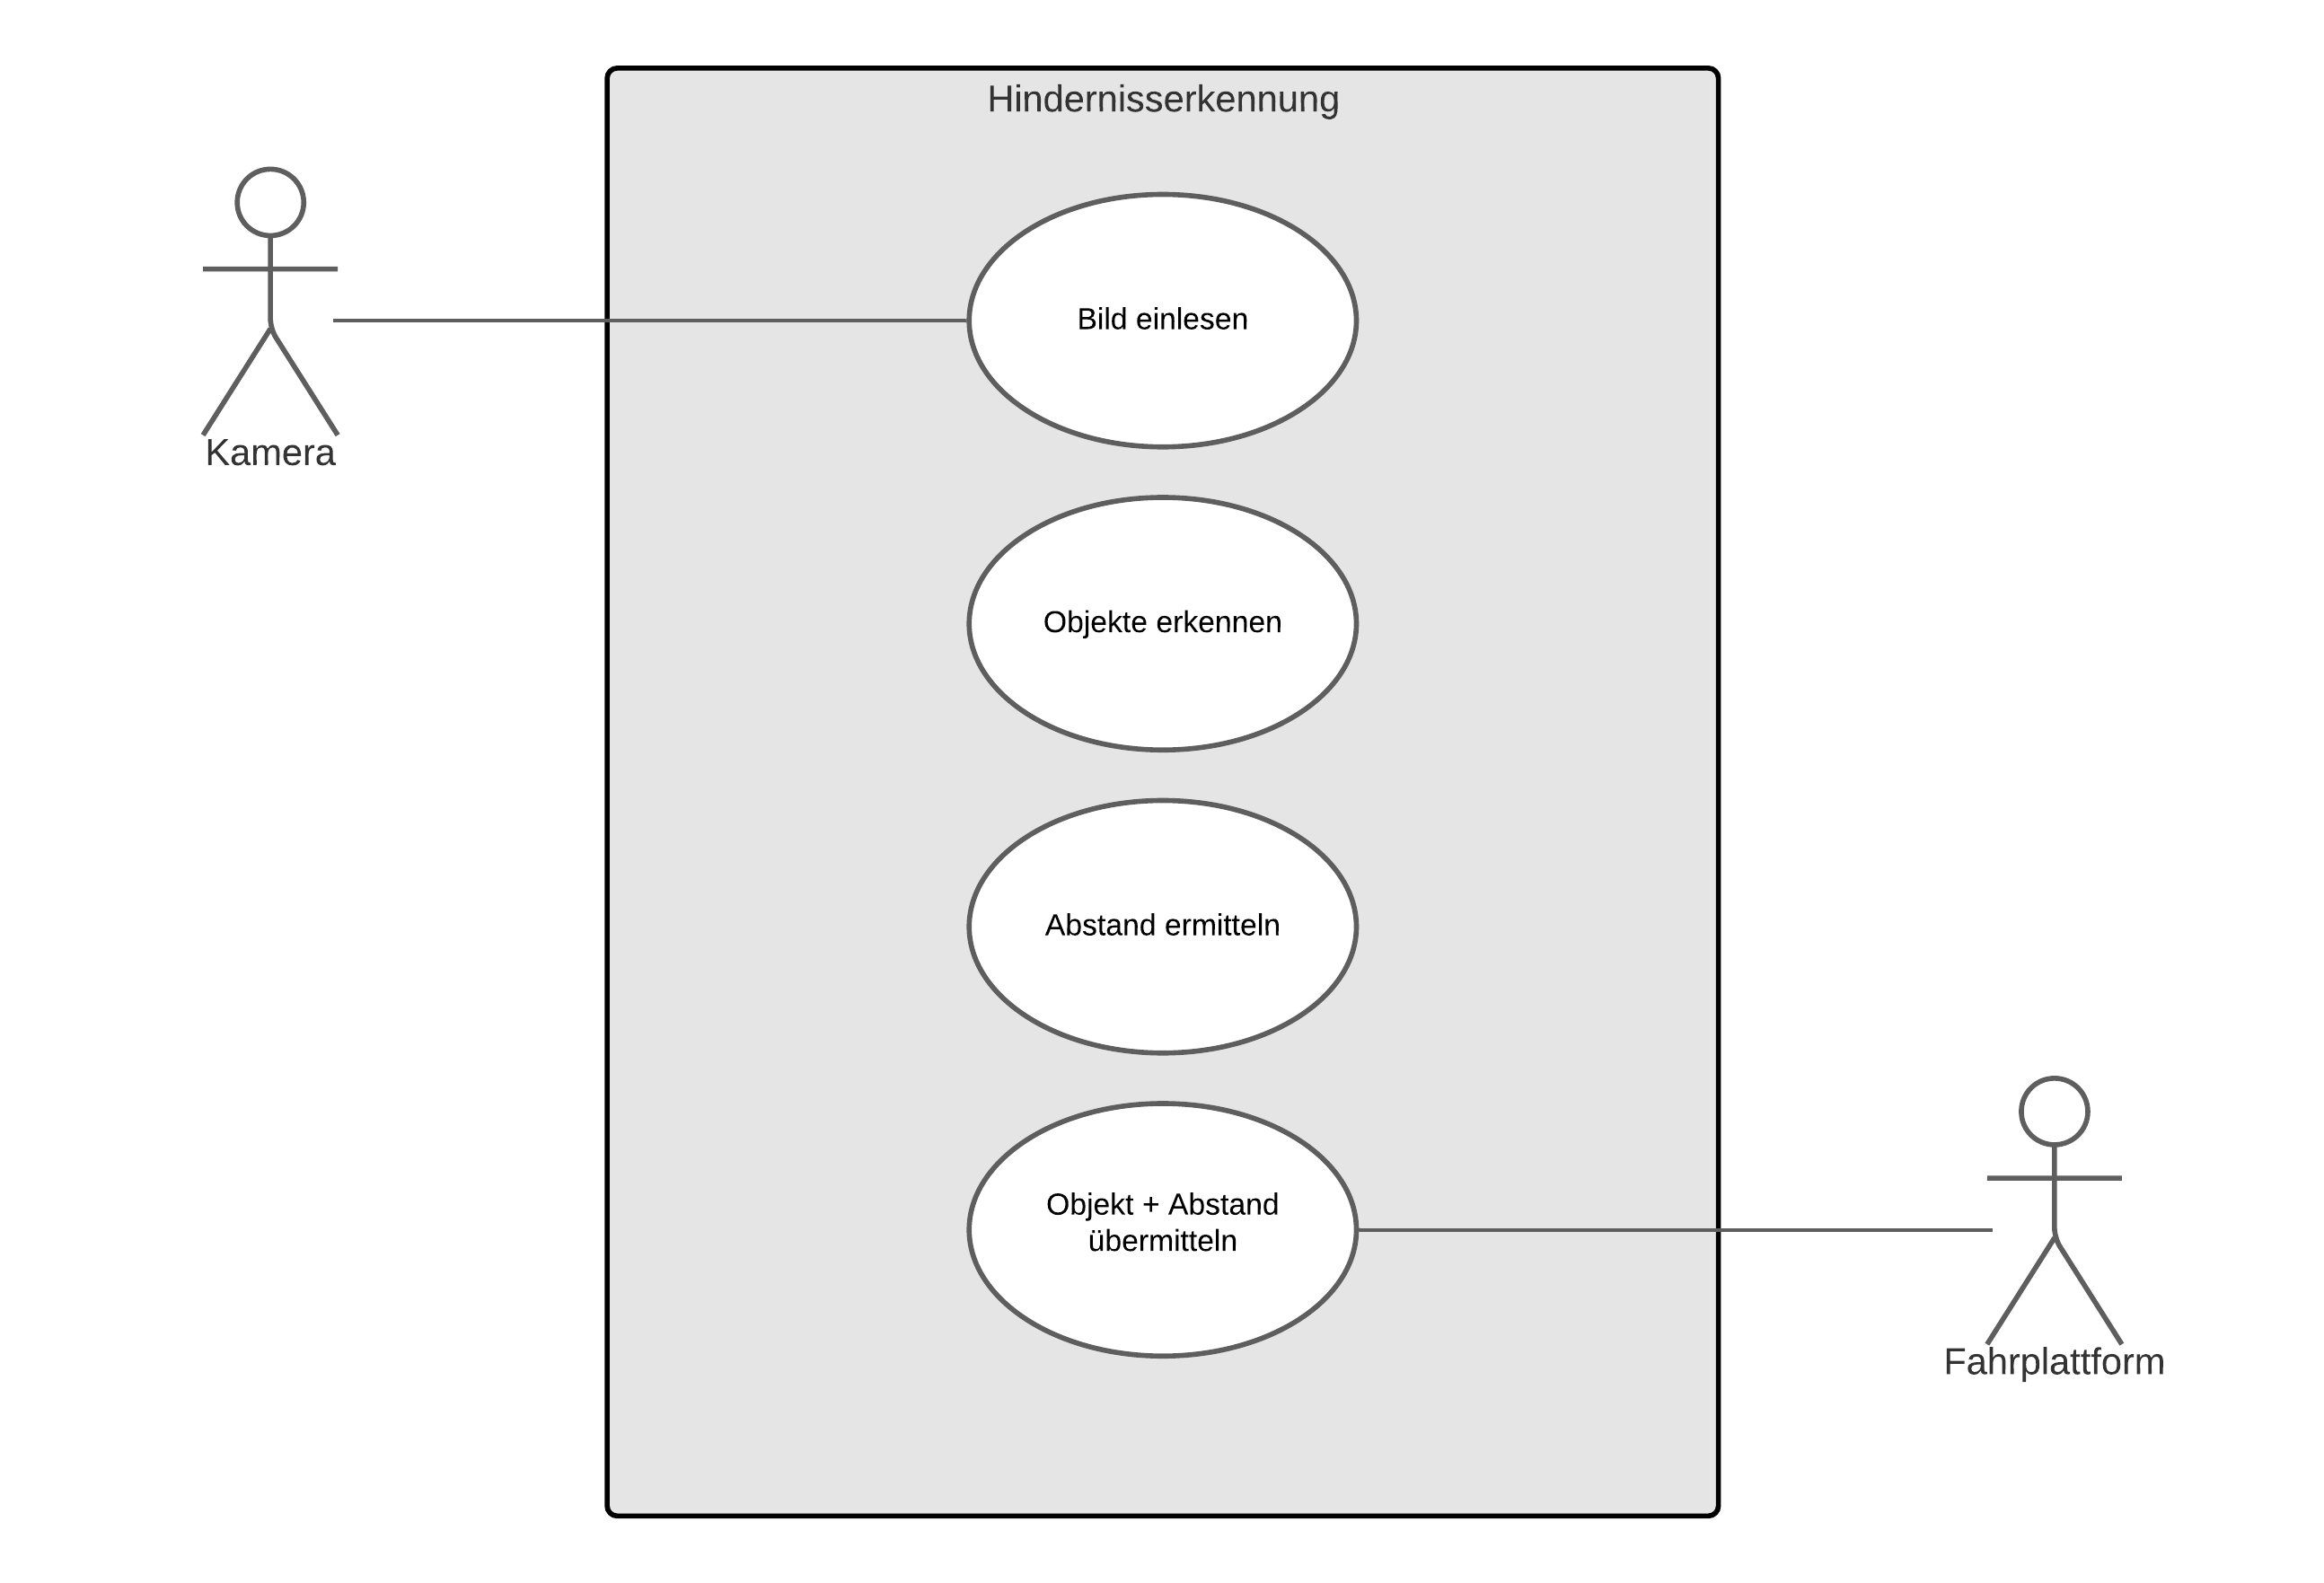
\includegraphics[width=1\textwidth]{chapters/cheatsheet/images/UseCaseNeu.png}
		\caption[HSV Farbraum 3D - Bildquelle: \cite{opencvfarbraum}]{3D \cite{opencvfarbraum}}
		\label{fig:hsv1}
	\end{subfigure}%
	\begin{subfigure}{0.7\textwidth}
		\centering
		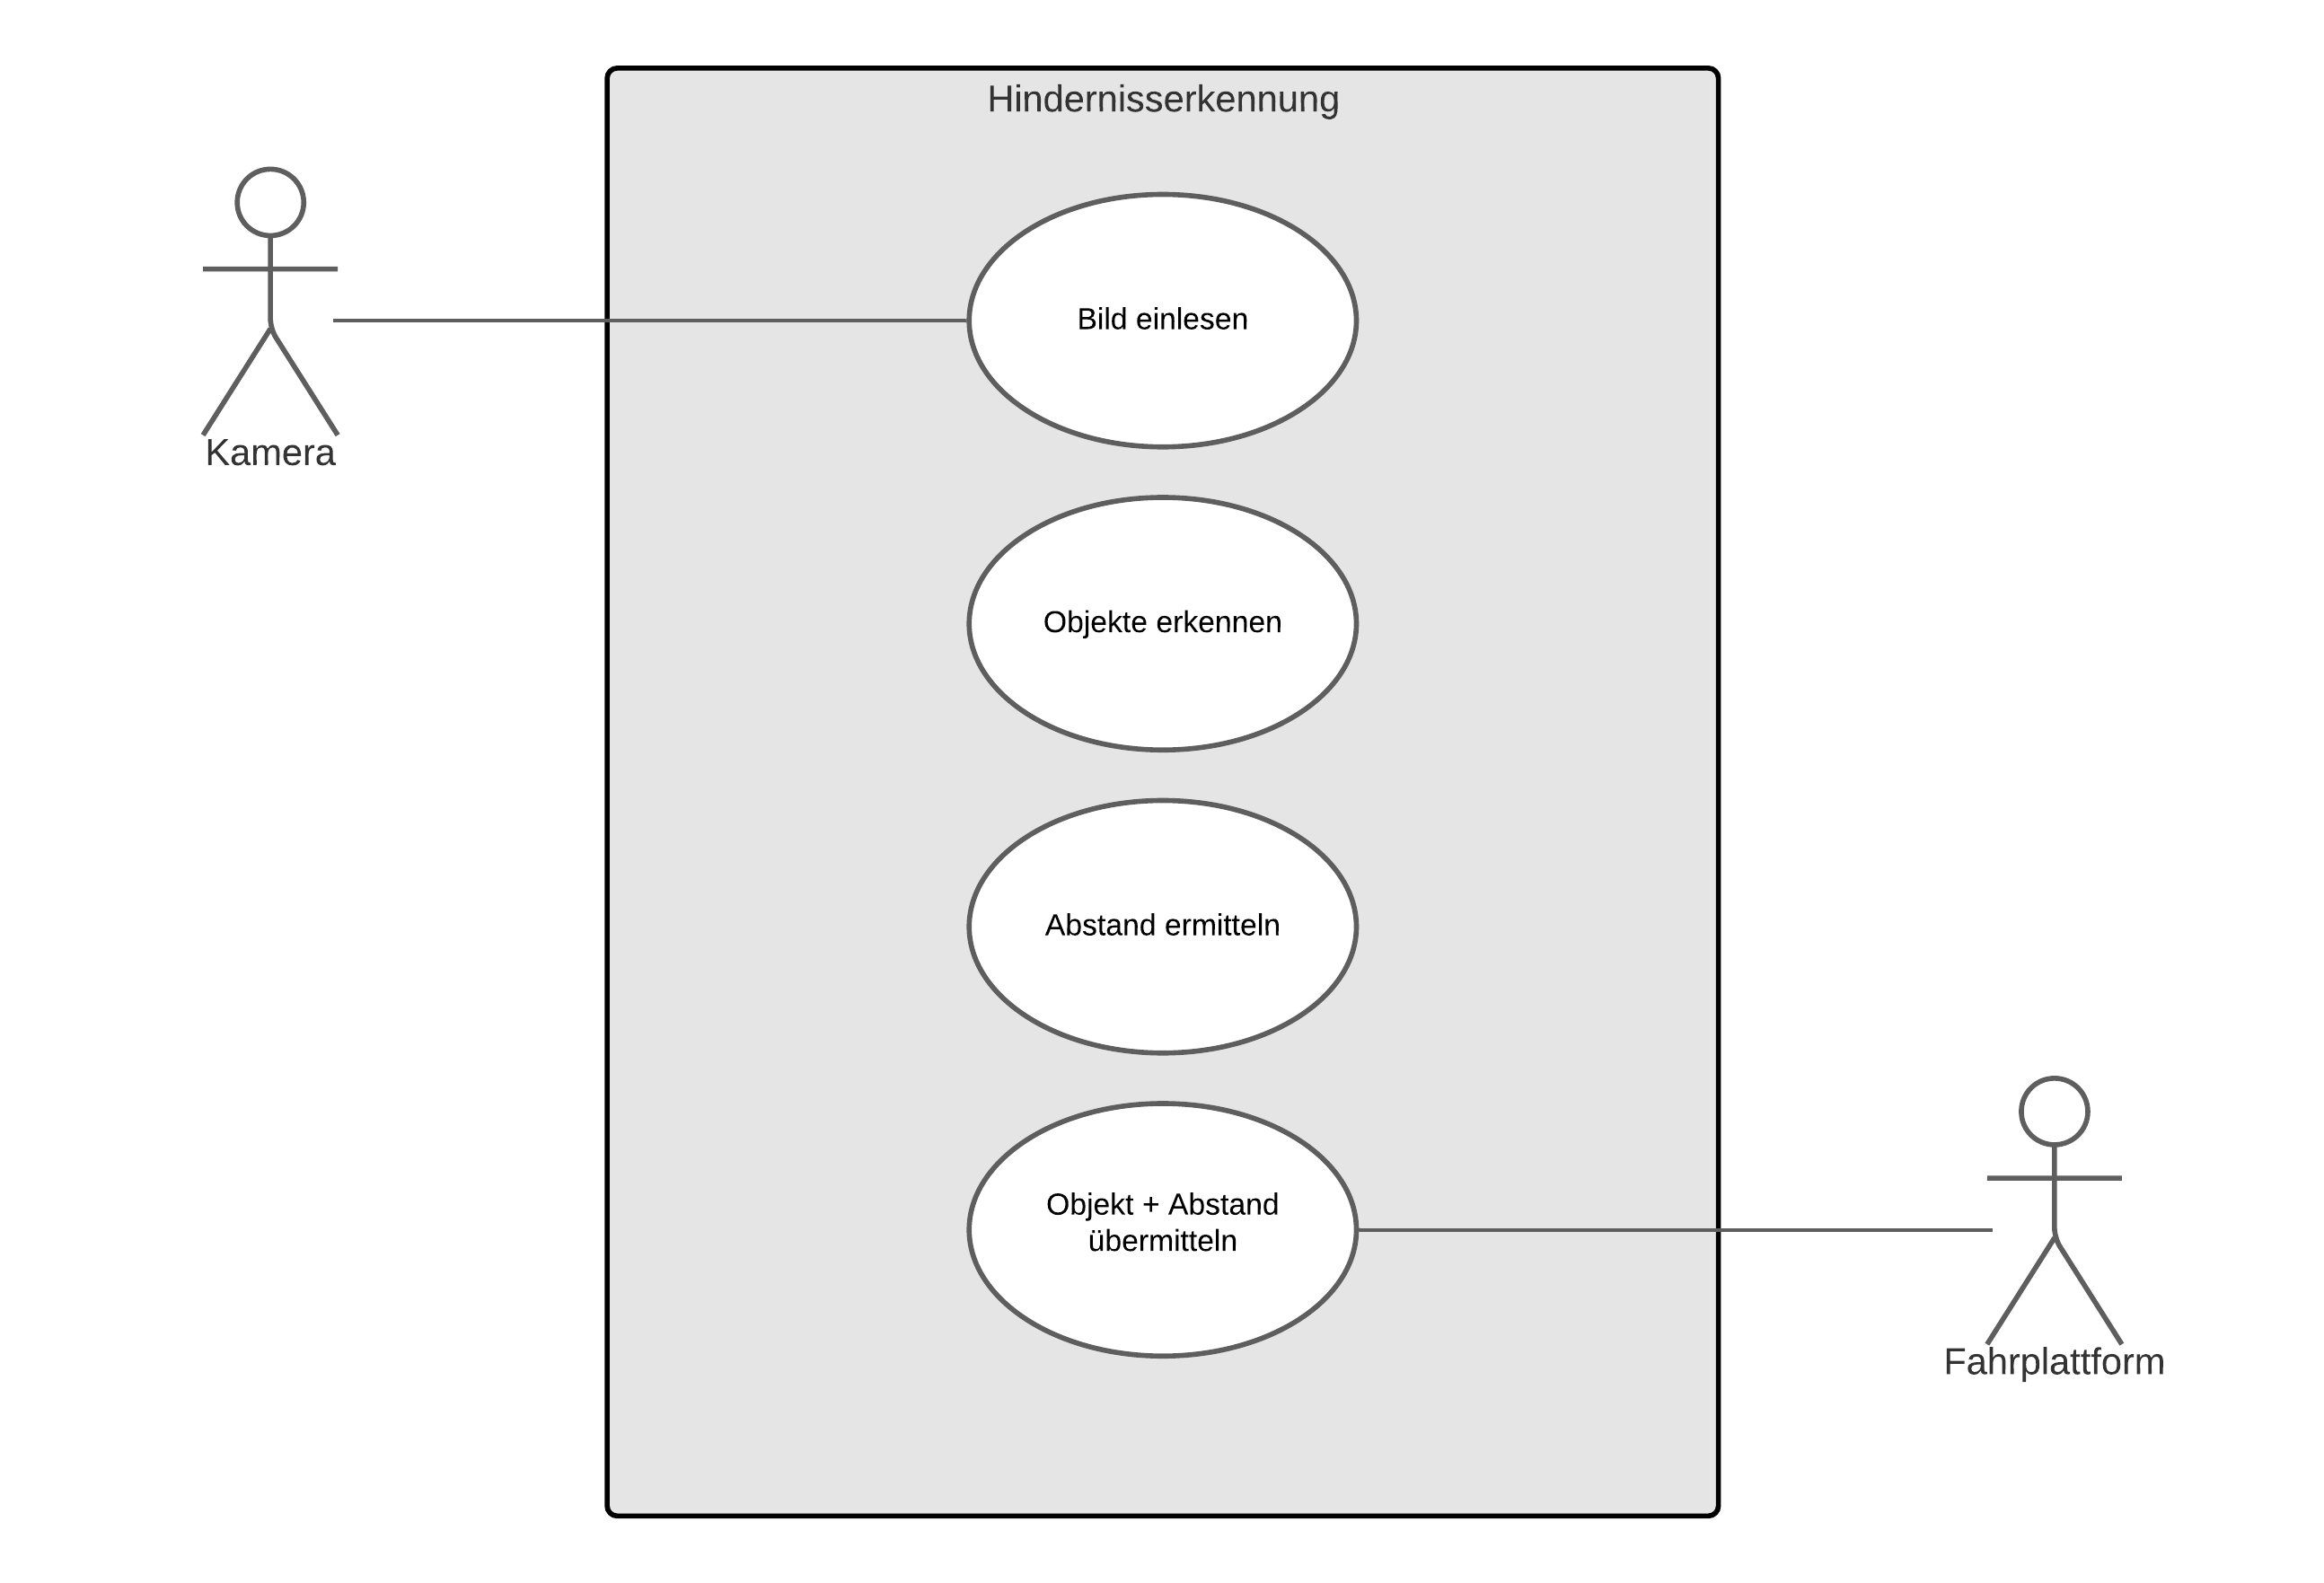
\includegraphics[width=0.8\textwidth]{chapters/cheatsheet/images/UseCaseNeu.png}
		\caption[HSV Farbraum 2D - Bildquelle: \cite{hsv1}]{2D \cite{hsv1}}
		\label{fig:hsv2}
	\end{subfigure}%
	\caption[HSV Farbraum - Bildquelle: \cite{hsv1}]{HSV Farbraum}
\end{figure}


\begin{figure}[H]
	\begin{subfigure}[t]{0.35\textwidth}	
		\centering
		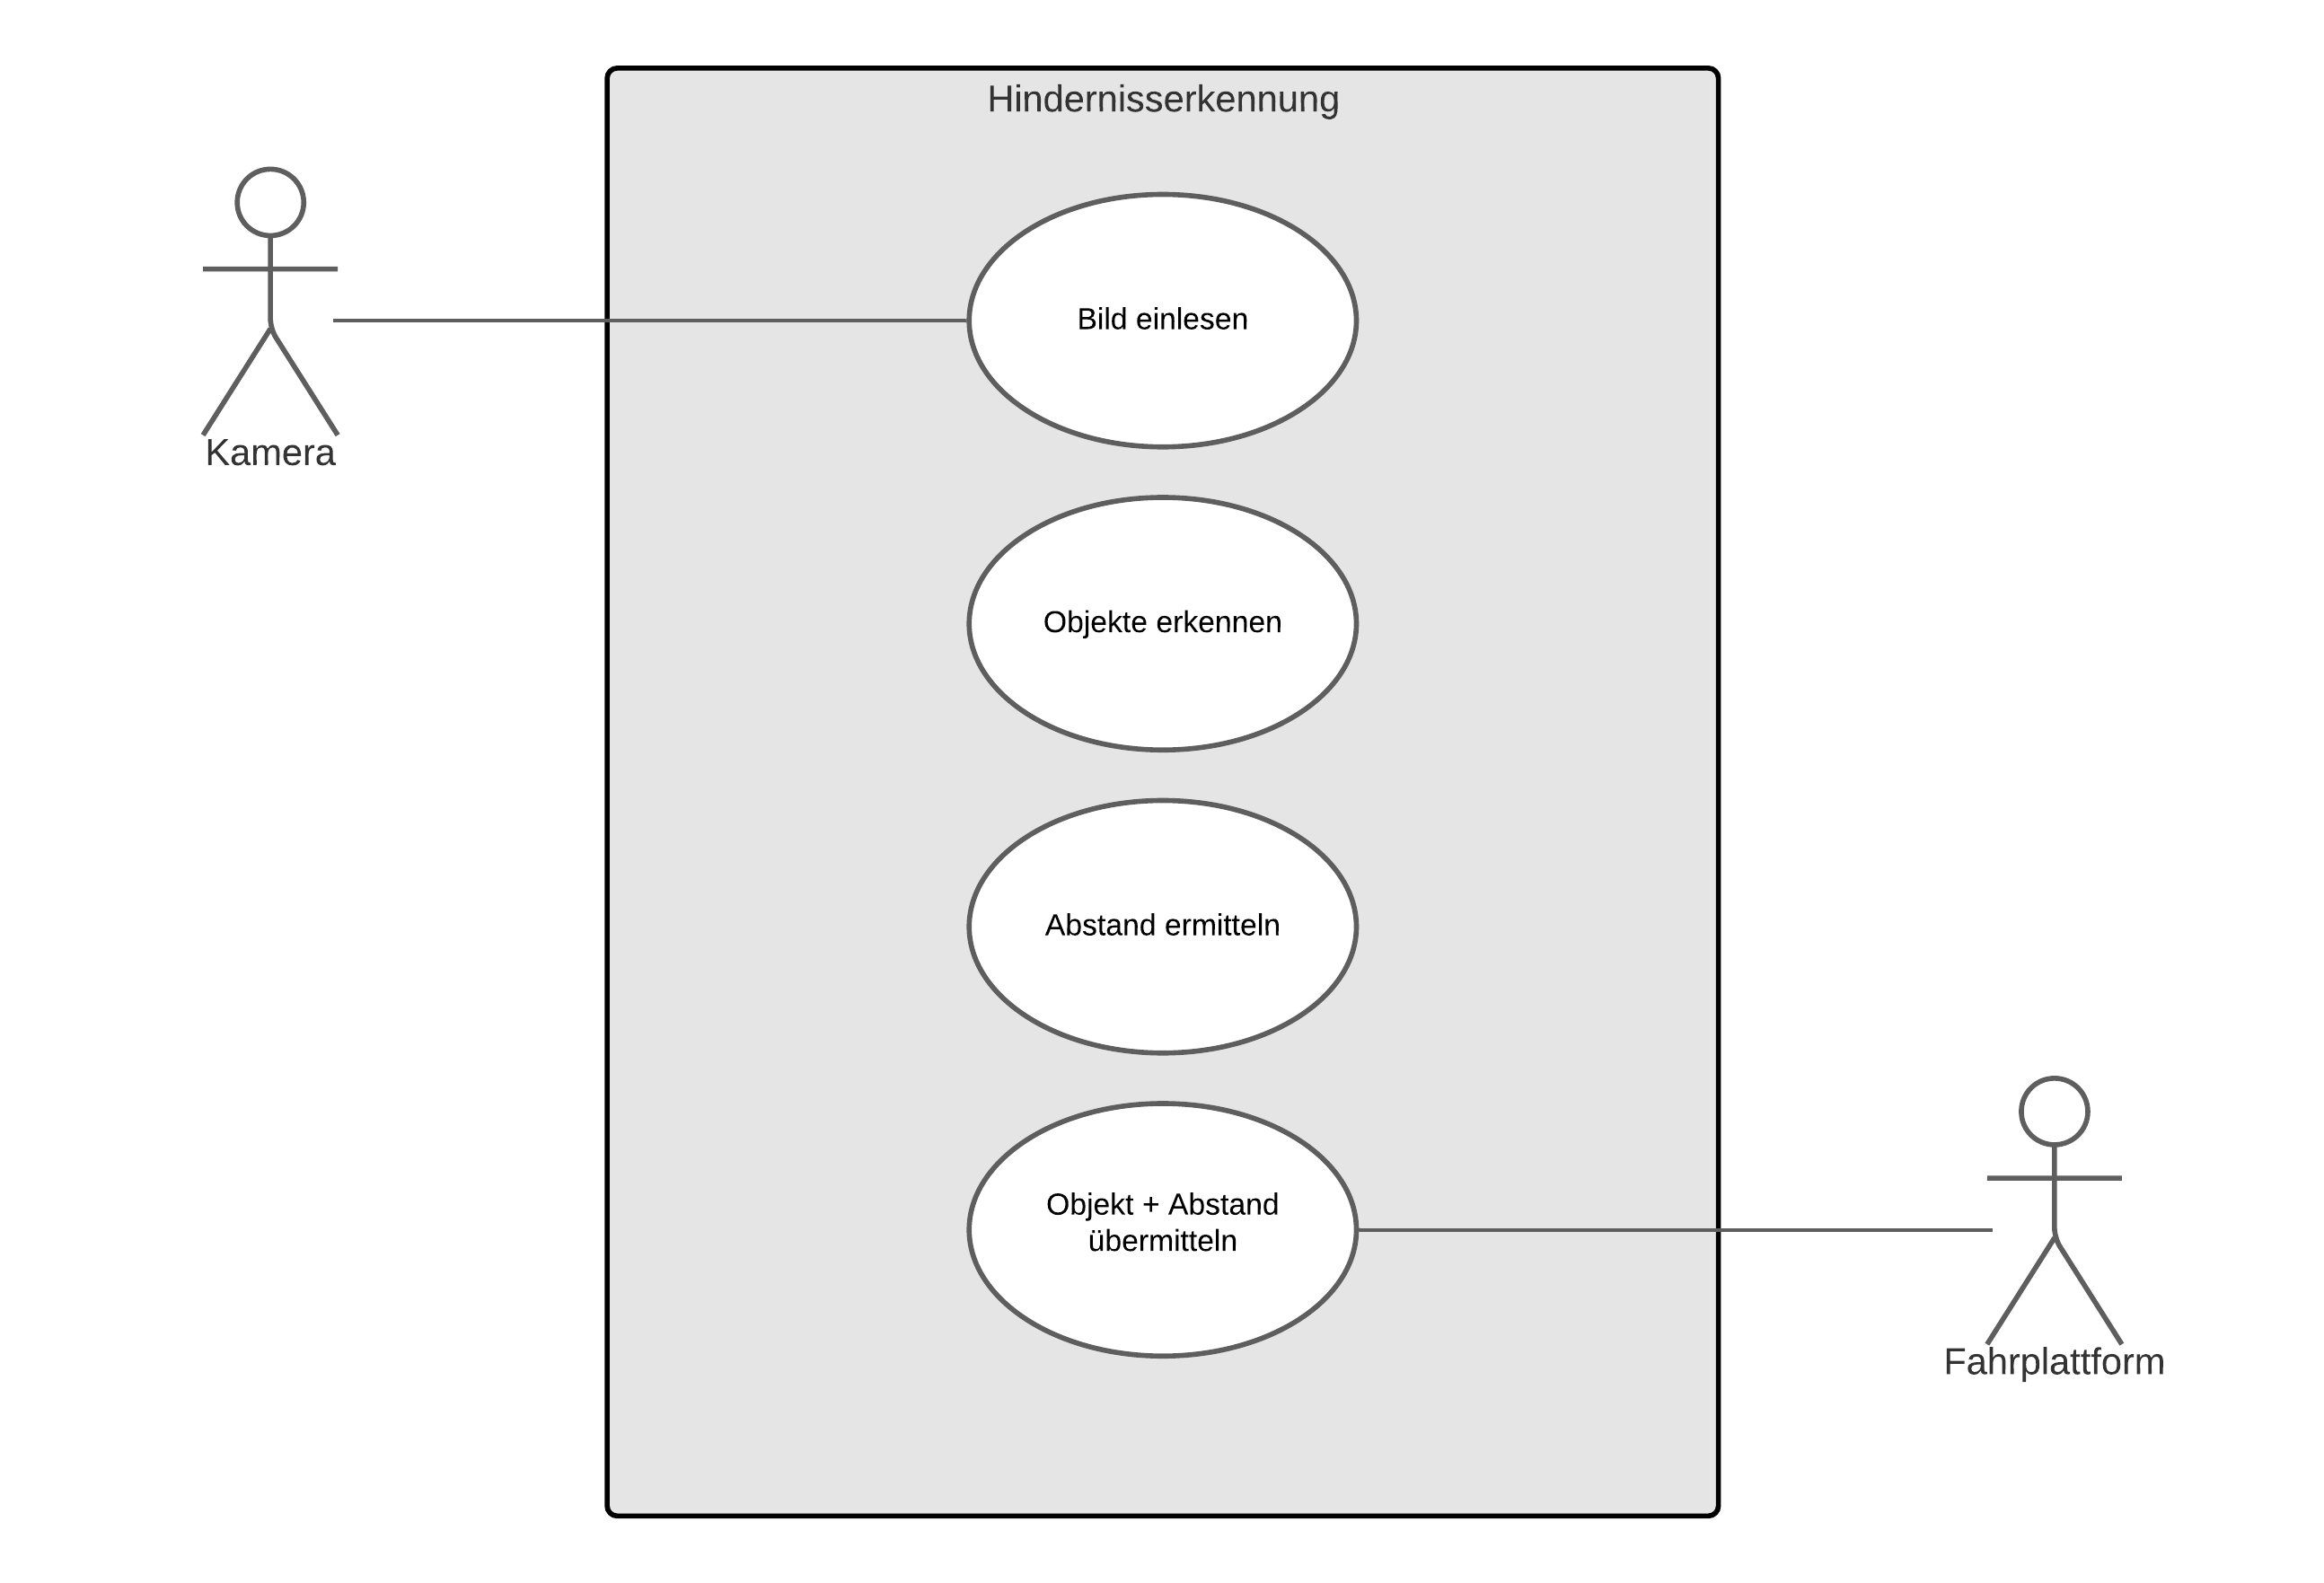
\includegraphics[width=0.9\textwidth]{chapters/cheatsheet/images/UseCaseNeu.png}
		\caption[Box mit höchster $p_{c}$ ist möglicherweise nicht der beste Treffer - Bildquelle: \cite{quickintro}]{Box mit höchster $p_{c}$\\ ist möglicherweise\\ nicht der beste Treffer \cite{quickintro}}
		\label{fig:rasteryolo1a}
	\end{subfigure}%
	\begin{subfigure}[t]{0.35\textwidth}
		\centering
		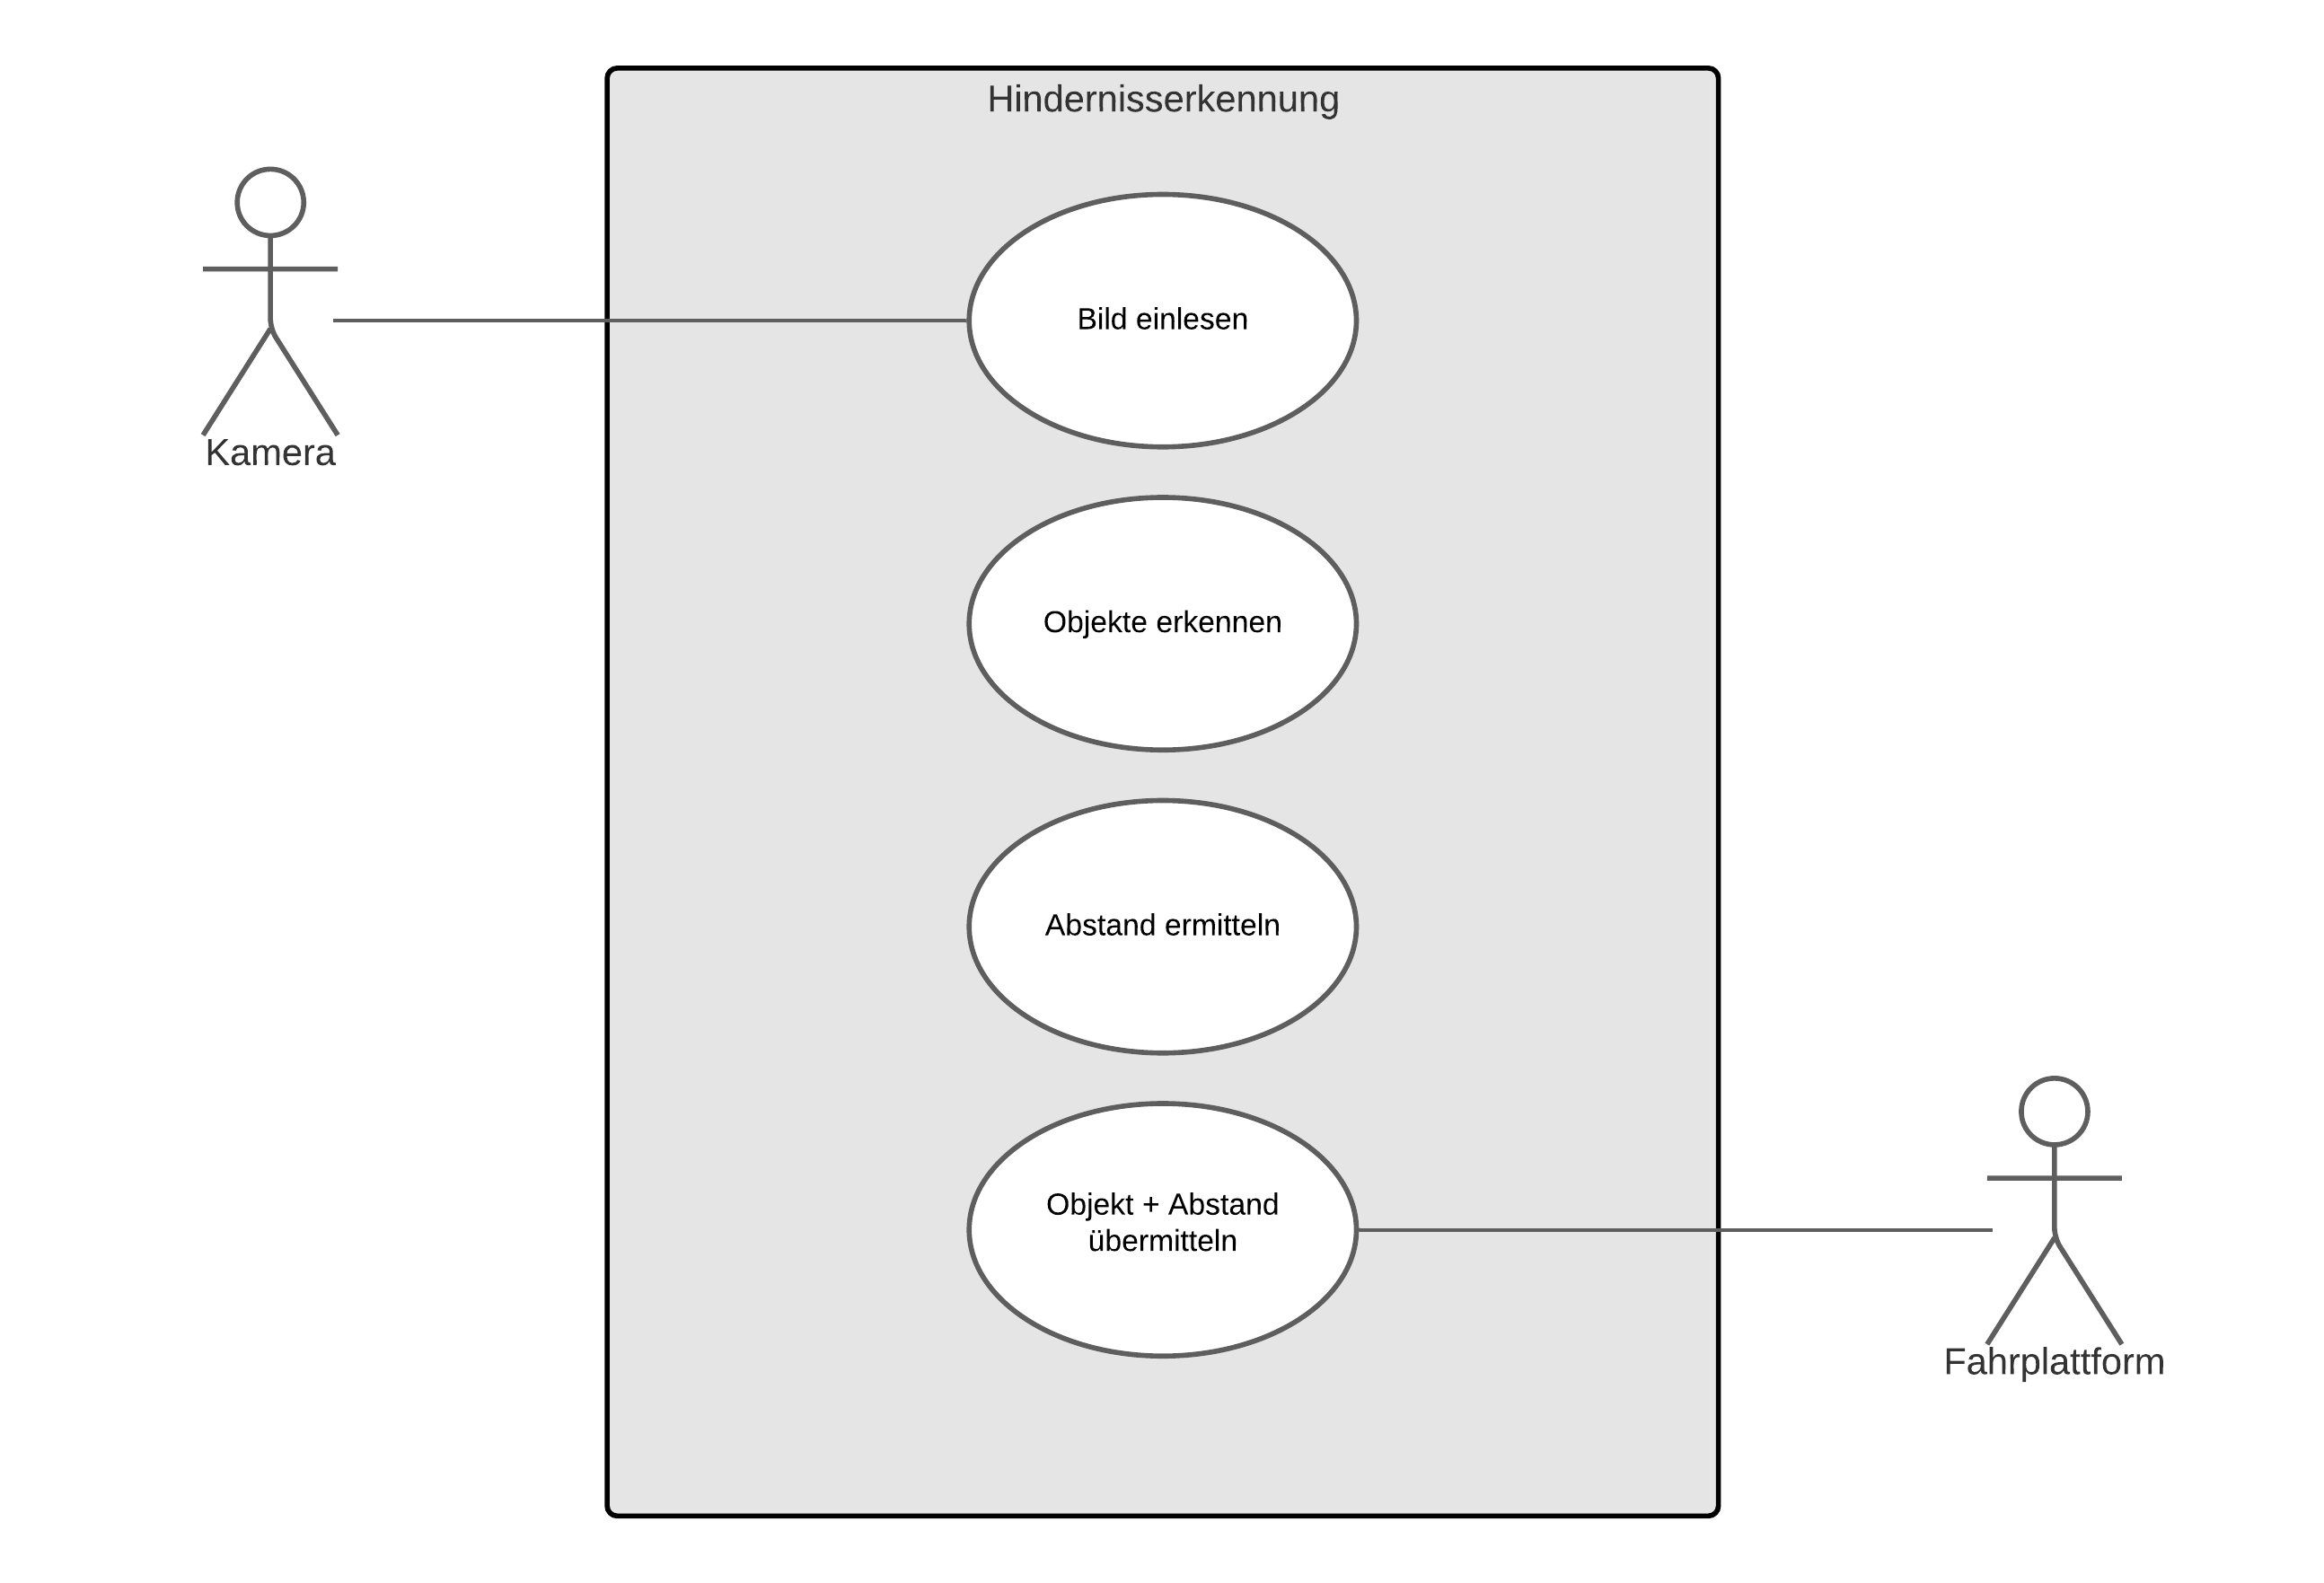
\includegraphics[width=0.8\textwidth]{chapters/cheatsheet/images/UseCaseNeu.png}
		\caption[Kann Objekte in der Nähe verwerfen - Bildquelle: \cite{quickintro}]{Kann Objekte in der\\ Nähe verwerfen \cite{quickintro}}
		\label{fig:rasteryolo1b}
	\end{subfigure}%
	\begin{subfigure}[t]{0.35\textwidth}
		\centering
		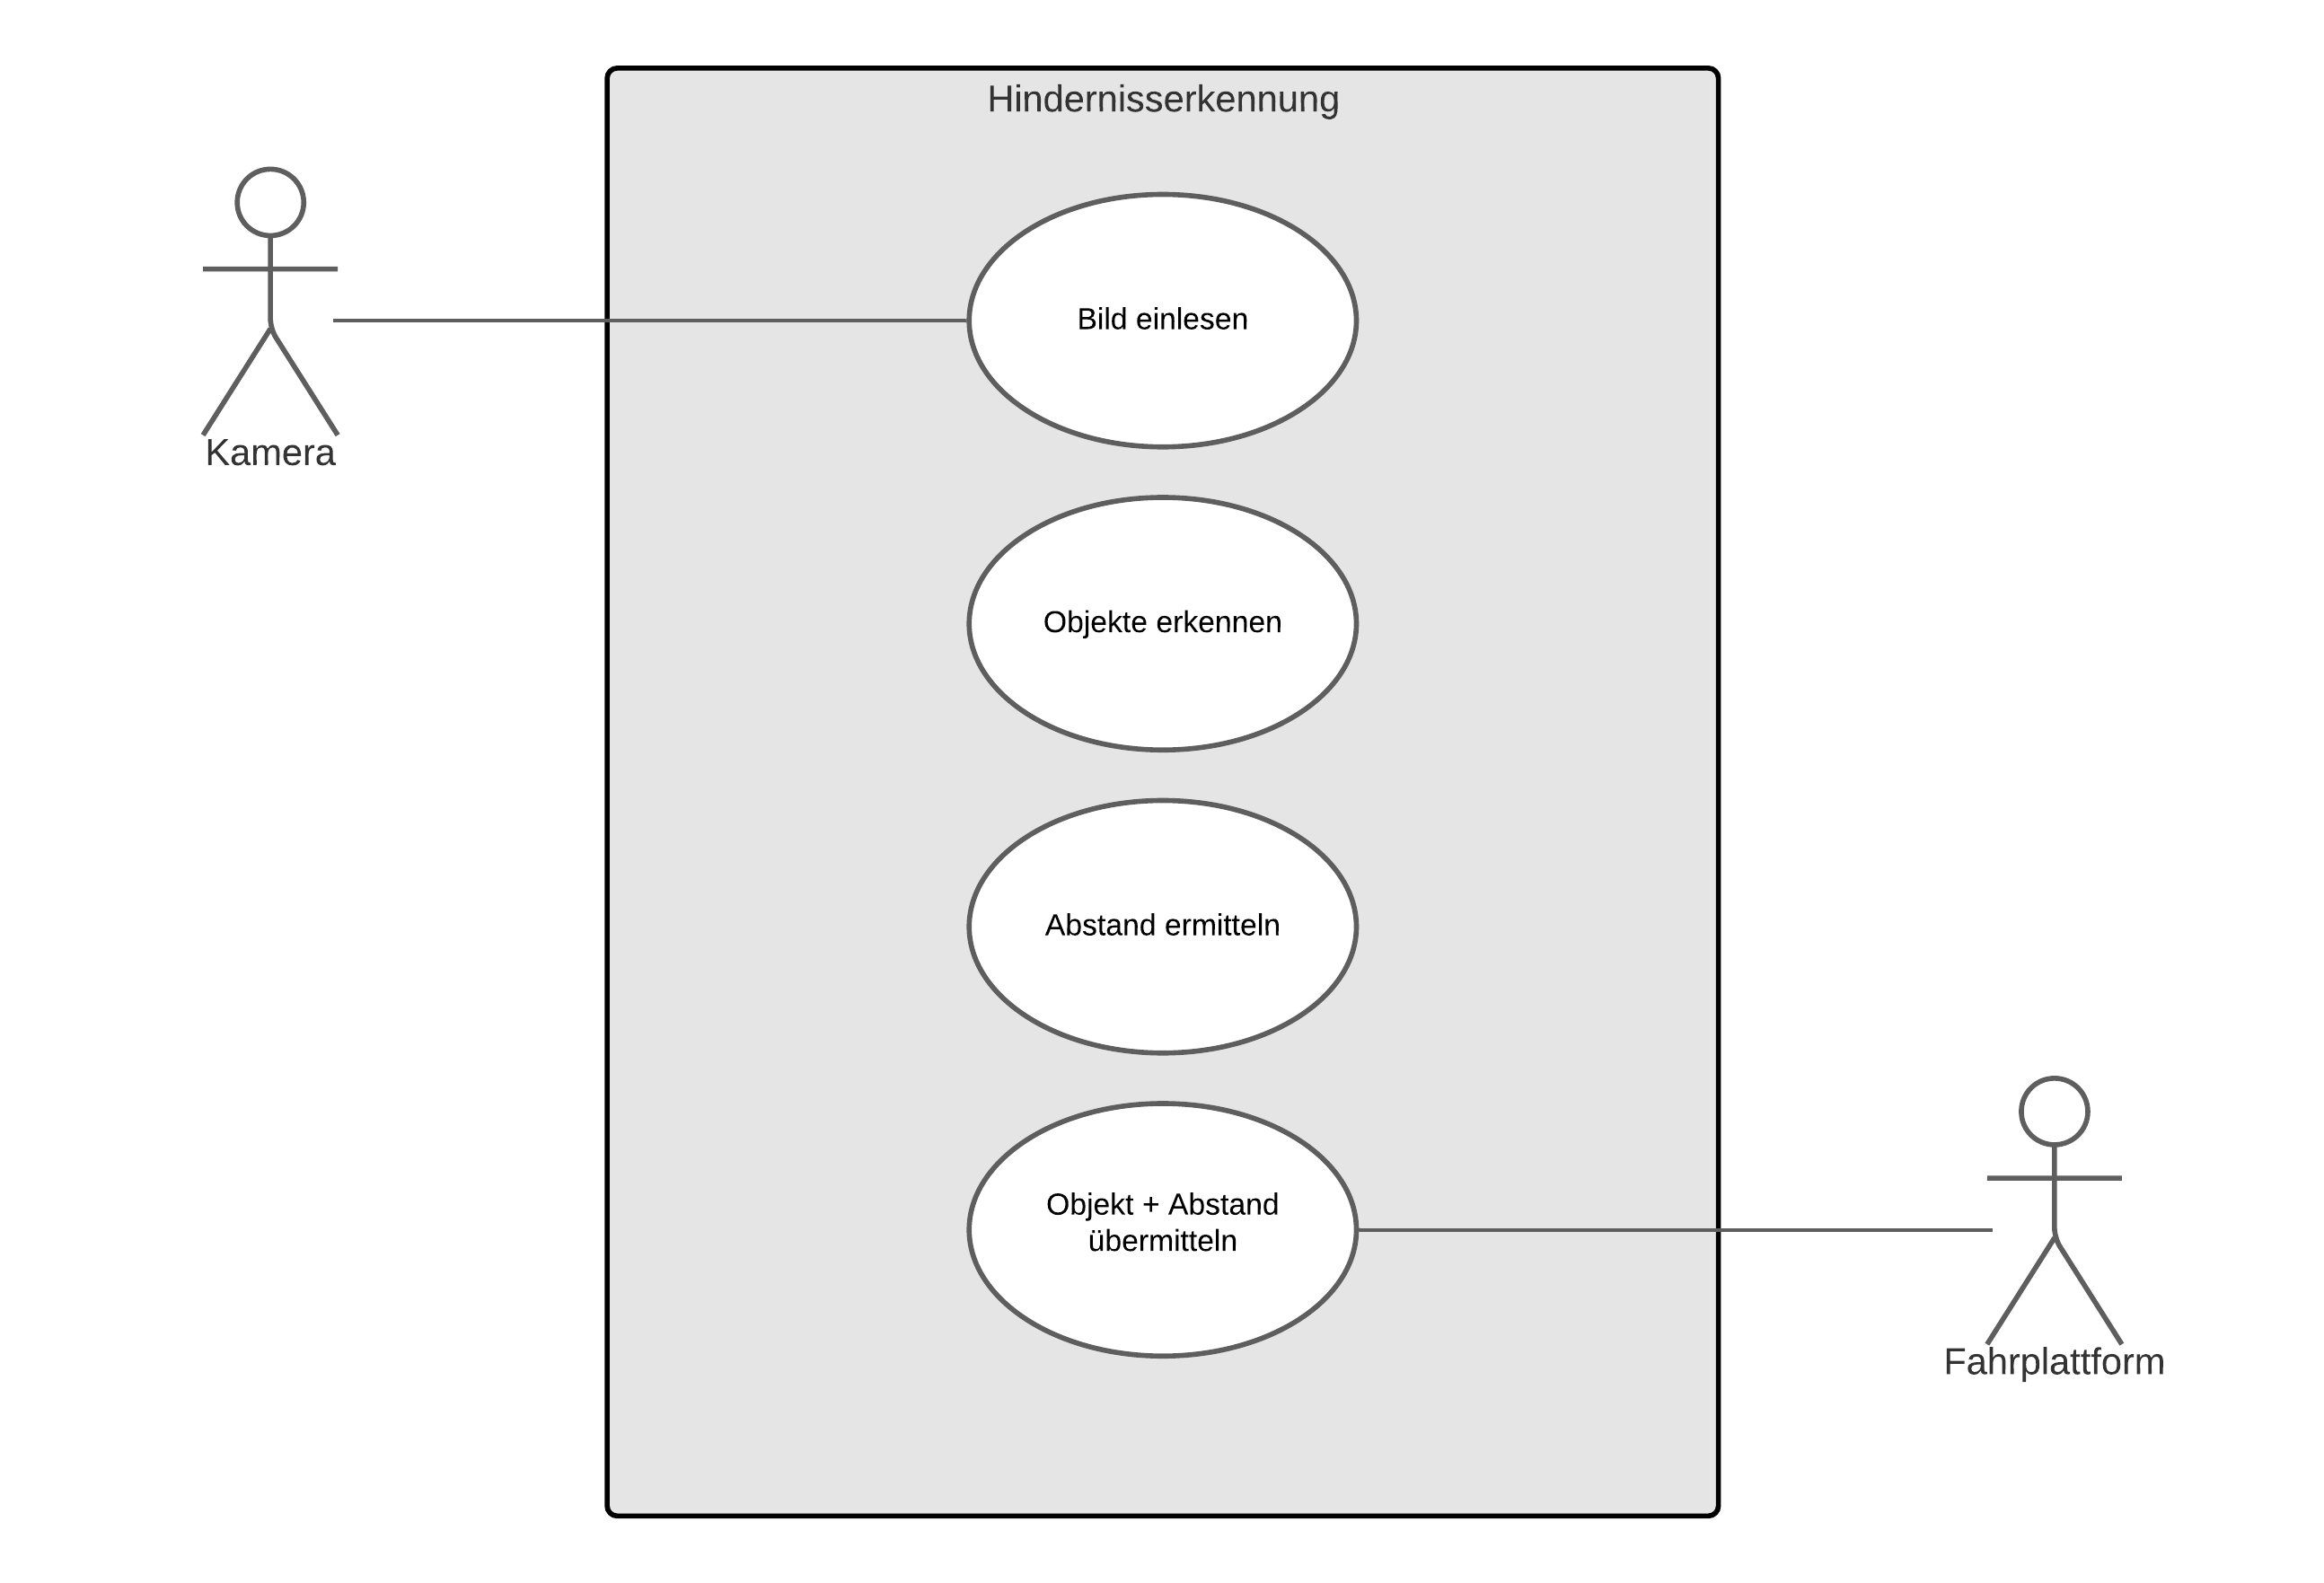
\includegraphics[width=0.9\textwidth]{chapters/cheatsheet/images/UseCaseNeu.png}
		\caption[Verwirft keine False-Positives - Bildquelle: \cite{quickintro}]{Verwirft keine\\ False-Positives \cite{quickintro}}
		\label{fig:rasteryolo1c}
	\end{subfigure}%
	\caption[Problemsituationen NMS - Bildquelle: \cite{quickintro}]{Probleme NMS}
\end{figure}


\begin{minipage}[h]{0.5\textwidth}
	\textbf{YOLO}\\
	Im YOLO-Format wird eine Bounding-Box durch vier Werte [x\_center, y\_center, width, height] dargestellt. Dabei sind x\_center und y\_center die normalisierten Koordinaten des Mittelpunkts der Bounding Box. Um die Koordinaten zu normalisieren, werden die Pixelwerte von x und y durch die Bildbreite x\_max beizehungsweise die Höhe y\_max geteilt.
	\vspace{1mm}
	
\end{minipage}
\begin{minipage}[h]{0.5\textwidth}
	
	\begin{figure}[H]
		\centering
		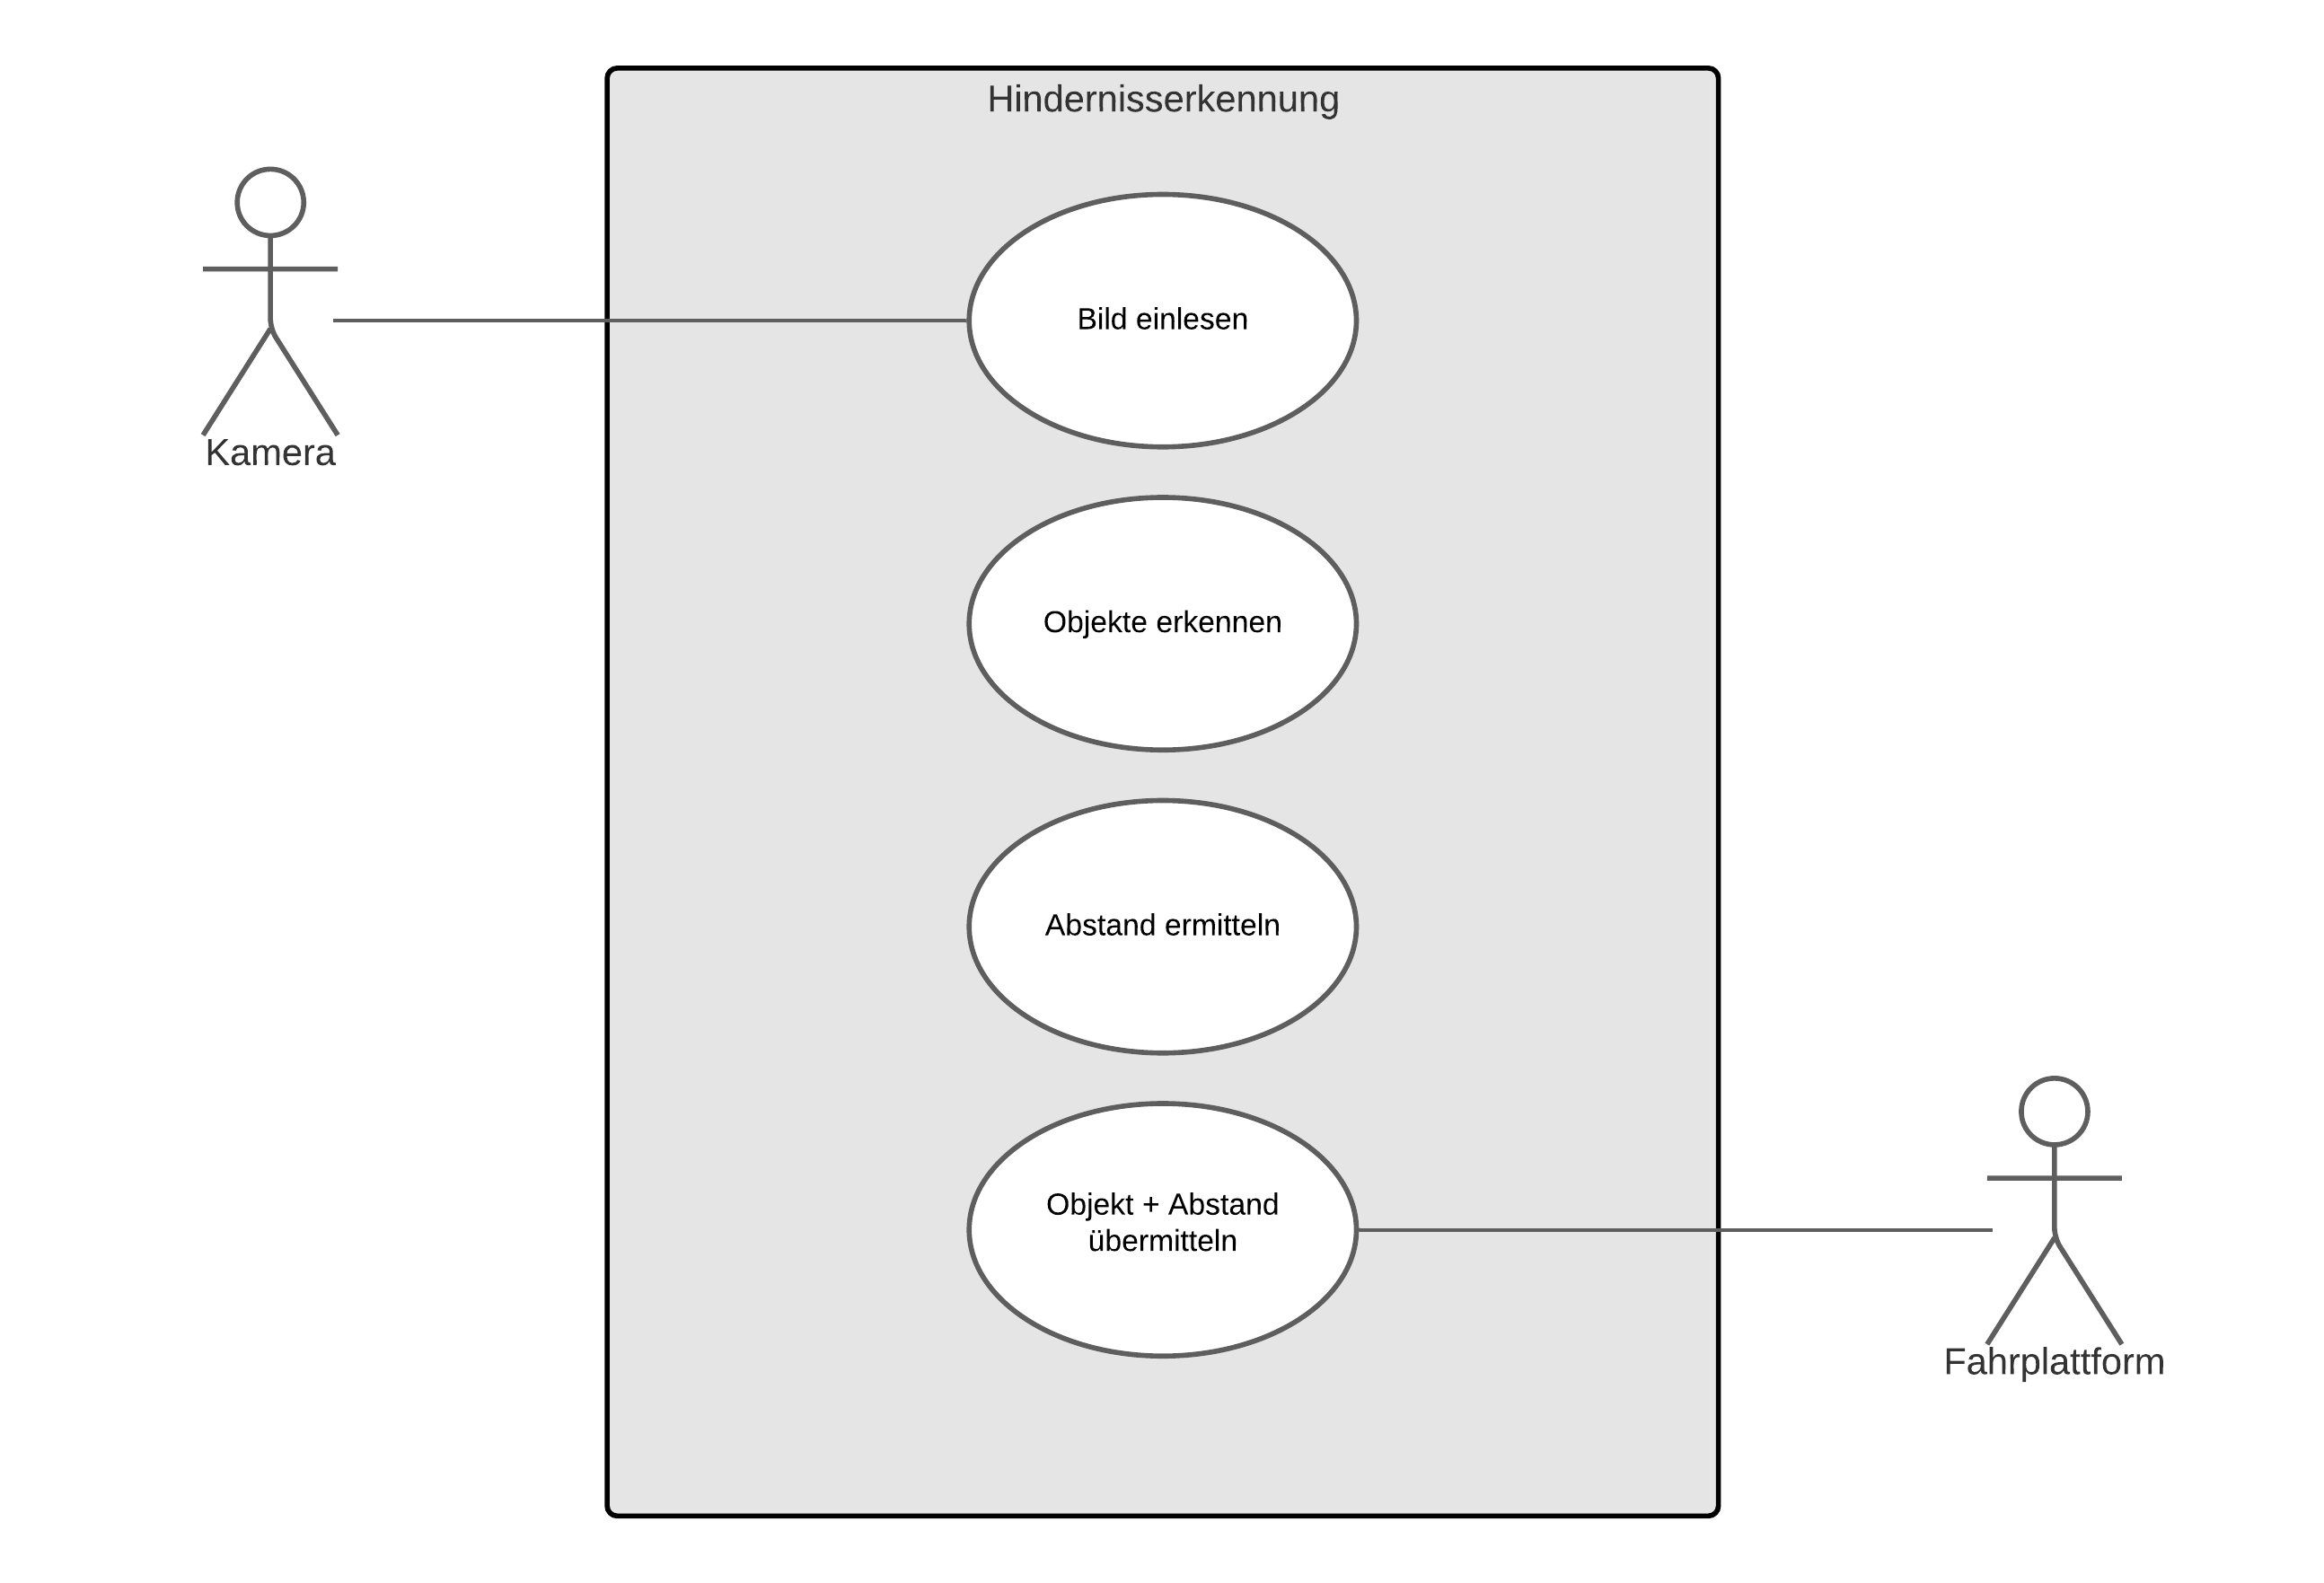
\includegraphics[width=1\textwidth]{chapters/cheatsheet/images/UseCaseNeu.png}
		\caption[Format YOLO - Eigene Darstellung]{Format YOLO}
		\label{fig:format2}
	\end{figure}
	\vspace{1mm}
\end{minipage}
\vspace{1mm}

\section{Formulas}

\begin{minipage}{.5\textwidth}
	\begin{equation}
		\mathbf{g(x, y)}_{x}=\left[\begin{array}{lll}+1 & 0 & -1 \\ +2 & 0 & -2 \\ +1 & 0 & -1\end{array}\right] * \mathbf{f(x, y)}
		\label{eq:sobel1}
	\end{equation}
\end{minipage}%
\begin{minipage}{0.5\textwidth}
	\begin{equation}
		\mathbf{g(x, y)}_{y}=\left[\begin{array}{ccc}+1 & +2 & +1 \\ 0 & 0 & 0 \\ -1 & -2 & -1\end{array}\right] * \mathbf{f(x, y)}
		\label{eq:sobel2}
	\end{equation}
\end{minipage}%




\begin{equation}
	\begin{alignedat}[b]{2}
		& & \zerotext{$\mathrm{~G} =\text{Gegenstandhöhe in Echt in cm}$} \\
		& d=\frac{f \cdot G}{B}& \zerotext{$\mathrm{~B} =\text{Gegenstandhöhe im Bild in Pixel}$} \\
		& & & \zerotext{$\mathrm{~d} =\text {Abstand in cm}$} \\
		& & \zerotext{$\mathrm{~f} =\text {Brennweite in Pixel}$} \\
	\end{alignedat}
\end{equation}




\section{Tables}
\begin{table}[H]
	\centering
	\begin{tabular}[H]{llp{5cm}}
		Augmenter & Parameter & Beschreibung \\ \hline
		& & \\
		Rotate &  $\pm$ 5\textdegree & Bilder werden zufällig bis zu fünf Grad nach links oder rechts um den Bildmittelpunkt gedreht.\\
		& & \\
		Linear Contrast & $\alpha$ = 0.5-1.5  & Erhöht oder verringert Kontrast der Bilder um den Faktor Alpha, der pro Bild zufällig aus einem Intervall gewählt wird.\\
		& & \\
		Motion blur & Kernel = 3x10, horizontal & Den Bildern wird eine horizontale Bewegungsunschärfe hinzugefügt.\\
		& & \\
		Flip & 50\%, horizontal & Bild wird mit einer Wahrscheinlichkeit von 50\% horizontal gespiegelt.\\
		
	\end{tabular}
	\caption{Funktionen der Augmentationspipeline}
	\label{tab:imgaugmenters}
\end{table}


\begin{table}[H]
	\centering	\begin{tabularx}{\textwidth}{|X|c|c|c|}
		\hline
		Phase:  & Median & Mittelwert & Standardabweichung \\ \hline
		Preprocessing: &  - &  - & - \\ \hline
		Inference: &  211 ms & 212 ms & 6 ms \\ \hline
		Postprocessing: &  19 ms & 35 ms & 158 ms \\ \hline
		Gesamt: & 230 ms & 247 ms & 158.11 ms \\ \hline
	\end{tabularx}
	\caption{Performancemessung YoloV5s Pytorch, Auflösung 640x640}
	\label{tab:performYoloV5PT_640}
\end{table}


\section{Code}

\begin{lstlisting}[caption=Training starten]
	%cd /home/$user/yolov5
	!python train.py --img 640 --batch 20 --epochs 600
	--data '../streetsigns.yaml'
	--cfg ./models/yolov5s.yaml
	--weights 'yolov5s.pt'
	--name yolov5s_streetsigns150521_results  --cache
\end{lstlisting}


%
% !TeX spellcheck = de_DE

\chapter{Questions}



\begin{todolist}
		\item[\done] Item1
		\item Item2
		\item[\wontfix] Item3
\end{todolist}

\end{document}
% % % % % % % % % % % % % % 
